\documentclass[11pt, twoside]{book}

%Title
\usepackage{comment}
% This command changes the font style where SLU promotes Arial
\newenvironment{myfont}{\fontfamily{phv}\selectfont}{\par}
% Math packages
\usepackage{steinmetz}
\usepackage{amsmath}
\usepackage{amssymb}
\usepackage{siunitx}
\usepackage{physics}
\usepackage{nicefrac}
% Image and float settings
\usepackage{graphicx}
\usepackage[font={small}]{caption}
\usepackage{subcaption}
\graphicspath{{./Figures/}}
\newsavebox{\largestimage}
\usepackage{float}
\usepackage{longtable}
% Tikz
\usepackage{tikzit}
\usetikzlibrary{scopes} 
\usetikzlibrary{backgrounds}
\usetikzlibrary{calc}
\usetikzlibrary{quantikz}
% Place images on top of page
\makeatletter
\setlength{\@fptop}{0pt}
\makeatother
%Glossary
%\usepackage[toc, acronym, nonumberlist]{glossaries}
% Page formatting
\usepackage[margin=1in]{geometry}
\usepackage{emptypage}
% Color package
\usepackage{xcolor}
\colorlet{shadecolor}{blue!10}
% Codes
\usepackage{listings}
\usepackage{pythonhighlight}
\lstset{columns=fullflexible}
\usepackage{spverbatim}
\usepackage{minted}
% Formatting of list items
\usepackage{enumitem}
% Dummy text
\usepackage{lipsum}
\usepackage{afterpage}
% Clickable links
\usepackage{hyperref}
\hypersetup{
    colorlinks=true,
    linkcolor=blue
}
% Remove indentation in paragraphs
\setlength{\parindent}{0pt}
\renewcommand{\baselinestretch}{1}
% Remove dots in TOC
\usepackage{tocloft}
\renewcommand{\cftdot}{}
% Parapgraph formatting
\usepackage{parskip}
\setlength{\parskip}{1em}
% Multiple rows and columns
\usepackage{multicol}
\usepackage{multirow}
% Headers and footers
\usepackage{fancyhdr}
\pagestyle{fancy}
\fancyhf{}
\fancyhead[L]{\leftmark}
\fancyhead[R]{\thepage}
\renewcommand{\headrulewidth}{1pt}

\input{Tikzit/sample.tikzdefs}
\input{Tikzit/sample.tikzstyles}

\usepackage[utf8]{inputenc}
\usepackage[english]{babel}
\usepackage{pdfpages}

\begin{document}
\pagestyle{empty}
%Cover page
\newgeometry{margin = 0in}
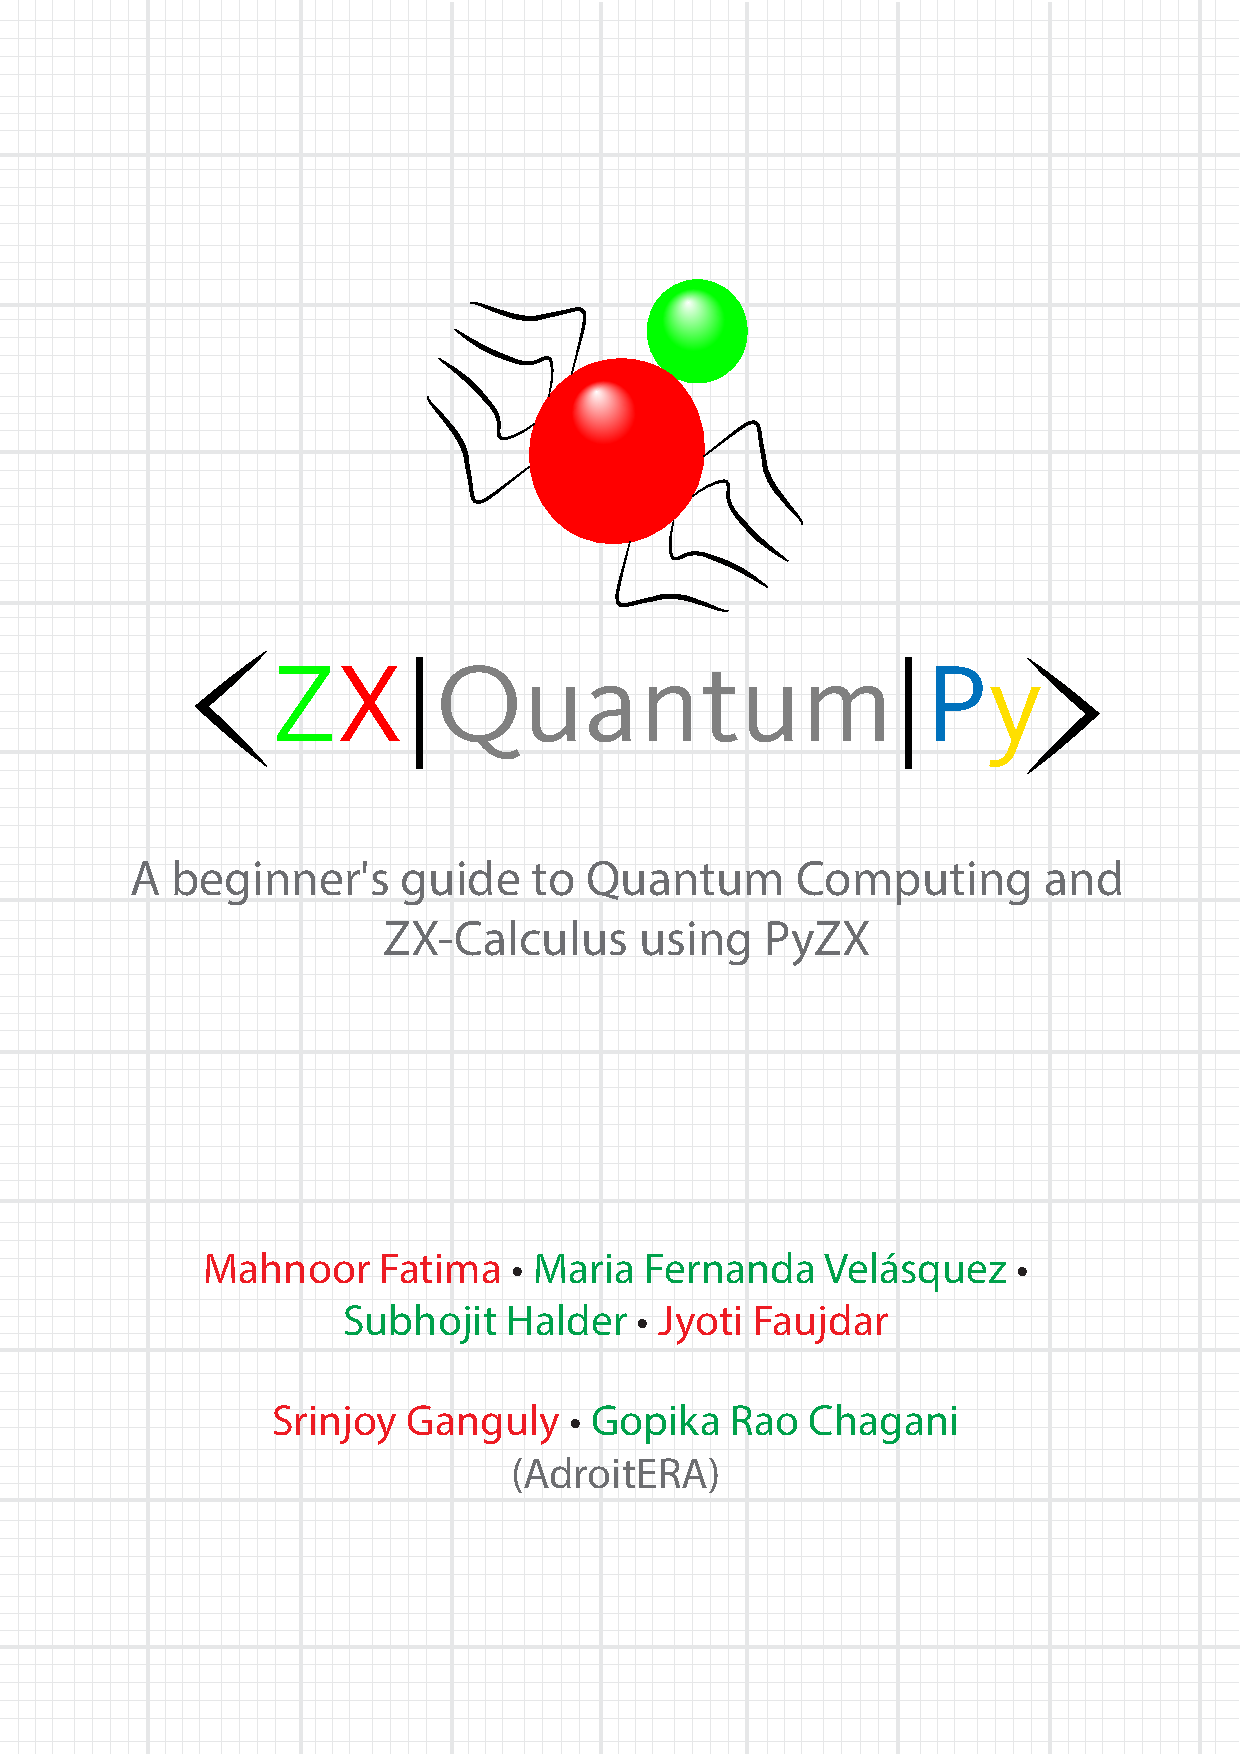
\includepdf[width = \textwidth]{cover}
\restoregeometry
% Title page
% To add this template to the main.tex file, just add the command "\include{titlePageSLU} after "\begin{docuemnt}" in the main.tex file

\newcommand{\thesisTitle}{ZX-Quantum-Py}
\newcommand{\thesisSubtitle}{A beginner's guide to Quantum Computing and ZX-Calculus using PyZX}
\newcommand{\credits}{30 hp}
%------------------------------------------------------------------------------
\begin{titlepage}
\thispagestyle{empty}

% Use this line of code if both SLU loggo and company/other institution loggo is desired. The positions are possible to change with the \hspace and \vspace syntax.


% Adds background picture. Delete code if no background picture is wanted.
\begin{comment}
\begin{tikzpicture}[overlay, remember picture]
\node[anchor=south west] 
     at (current page.south west)
      {\includegraphics[width=\linewidth]{Figures/recreational_exp/experiment_pics/led pattern.jpg}};
\end{tikzpicture}
\end{comment}

\hspace{2cm}
\centering
\vspace{4cm}
\par
\noindent
% \rule[0.3cm]{\linewidth}{1pt}
\begin{Huge}
{\textsc{\thesisTitle}}\\
\end{Huge}
\vspace{0.6cm}
\begin{Large}
\textsc{\thesisSubtitle}\\
\end{Large}
\vspace{0.9cm}
\rule[0.3cm]{0.2\linewidth}{1pt}

\vspace{3cm}

\noindent
\Large

Mahnoor Fatima\\
Maria Fernanda Velásquez\\
Subhojit Halder\\
Jyoti Faujdar\\
Srinjoy Ganguly (AdroitERA)\\
Gopika Rao Chaganti (AdroitERA) 
\end{titlepage}

\cleardoublepage

%-----------------------------------------------------------------------
%-----------------------------------------------------------------------
\pagestyle{fancy}
\setcounter{page}{1}
\pagenumbering{roman}

\tableofcontents
\chapter*{Acknowledgements}
\addcontentsline{toc}{chapter}{Acknowledgement}

We would like to extend our heartiest gratitude to our supervisors, Srinjoy Ganguly and Gopika Rao Chaganti, for providing us the opportunity to work on this project and for their constant mentorship, support, and guidance throughout the process.

We would also like to thank the QResearch Department, QWorld, for organising QIntern and for sponsoring our research project. Special thanks to Adam Glos and ‪Zoltán Zimborá for coordinating this program.
\chapter*{Preface}
\addcontentsline{toc}{chapter}{Preface}
\fancyhead[L]{Preface}
\lipsum
%-----------------------------------------------------------------------
\setcounter{page}{1}
\pagenumbering{arabic}
\fancyhead[L]{\leftmark}
\newpage
% % Chapters
\chapter{Introduction to Vectors}
% Alternate title: Vectors and their Mathematical Operations

{
\begin{center}
\fcolorbox{black}{shadecolor}{%

    \parbox{\textwidth}
    {%
        \small
        {
            This chapter is a basic introduction to vectors their mathematical operations. If you have already studied them, feel free to proceed to the next chapter!
        }
    }%
}
\end{center}
}

Whenever we want to define a quantity, we use numbers. For instance, if someone asks you how many candies you have, you can answer them in forms of numbers, say 1, 5, or 100. Numbers let you have a concrete idea about the amount of things. Thus, if you know that you have 5 candies and your sibling has 2, you can be sure that you have more candies than your sibling (yay!). The number which describe the 'quantity' of something is called its \textbf{magnitude}.

In science, we call all such things \textbf{scalar}. Because of this, we can say that a scalar is a quantity that can be described alone by its magnitude.

Let's take another example now. Suppose someone is asking you how far your school is from your home. You will make a nice guess and again answer in some sort of number, say 1 mile or 2 kilometers. That's all good -- no one will want you to \textit{measure} the whole distance on your own anyway. But there's still a problem. Even if we know that the school is 1 mile away from your home, this does not \textit{completely} describe the location of the school, because the school could either be in the north, south, east, or west of your home -- or anywhere in between. Hence, magnitude alone is not enough to describe the position of your school.

\begin{figure}[ht!]
    \centering
    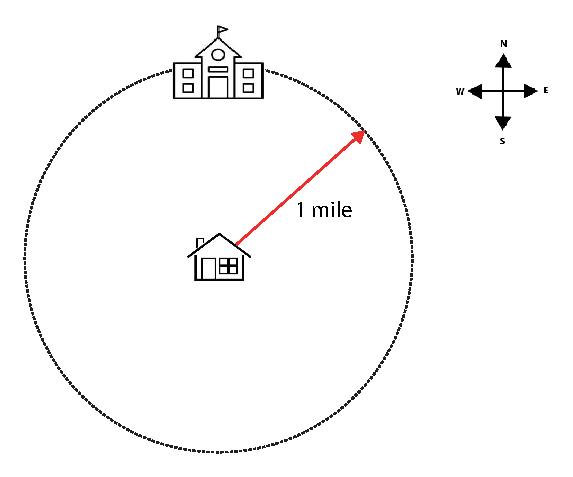
\includegraphics[scale = 0.7]{direction.eps}
    \caption{The problem faced with describing the position of the school from home. Every point on the circle is 1 mile away from the home, so saying 'My school is 1 mile away from home' is not enough; you need to tell the direction as well. In this figure, the direction is north.}
    \label{fig:direction}
\end{figure}

This problem demands that we add \textbf{direction} to our description as well. Hence, if you say that your school is 1 mile north from your home, this will completely describe the location of your school from your home. That is, we can say that position is completely described by both magnitude and direction. 

These quantities are called \textbf{vectors}. Thus, a vector is a physical quantity that is completely described by its magnitude and direction (and please keep this in mind; vectors will be your best bud to understand the next chapters!).

All the physical quantities are either scalars or vectors, about which you will study in your high school physics. But for now, this much description will be sufficient for the rest of the book.

\section{Description of Vector}
Just like we use numbers to describe scalars, we have different systems to describe vectors. 
\subsection{Polar Representation}
I'll be referring back to Fig. \ref{fig:direction}. Let's look at it from a different perspective. In the image, the magnitude of the position is given as the radius of the circle (in our case: 1 mile). So, all we need to do is describe the direction. For that, we will use angles. Suppose we take east as 0\si{\degree}. In that case, north will be described as 90\si{\degree} away from it. Thus, in polar representation, our position vector can be written as $1\phase{90\si{\degree}}$ mile. This is shown in Fig. \ref{fig:polar}.

\begin{figure}[!ht]
    \centering
    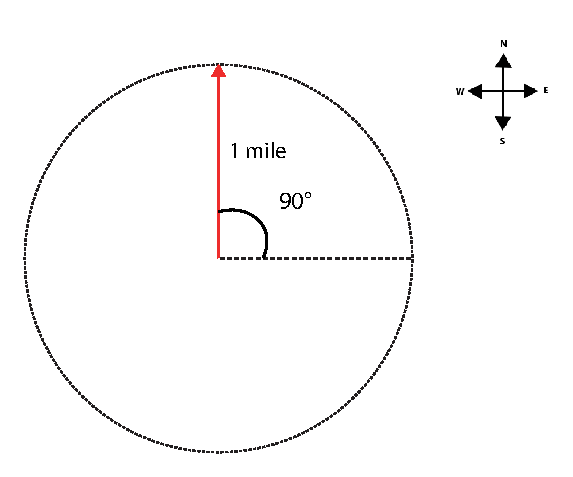
\includegraphics[scale = 0.8]{polar.eps}
    \caption{Redefining Fig. \ref{fig:direction} to show that the position vector can be represented with a radius and an angle, otherwise known as the polar representation of vectors. The images of house and school have been removed for convenience}
    \label{fig:polar}
\end{figure}

Generally speaking, the polar representation of a vector comprises a magnitude $r$ and an angle $\theta$; the vector itself is written as $r\phase{\theta}$.

\subsection{Rectangular Representation}
% write about (x, y) coordinates
Let's look back at Fig. \ref{fig:direction}. In fact, let's bring it on an x-y plane as shown in Fig. \ref{fig:rect-vec}. Here, we can see that the coordinates of the school are (0,10) if we consider one big box (marked by a slightly bolder grey line on the grid) as 0.1 mile. We can write this in vector notation as 10 $\hat{y}$ miles. Here, $\hat{y}$ simply means that this is the y-component of the vector. The meaning of the hat will be described shortly.

\begin{figure}[!ht]
    \centering
    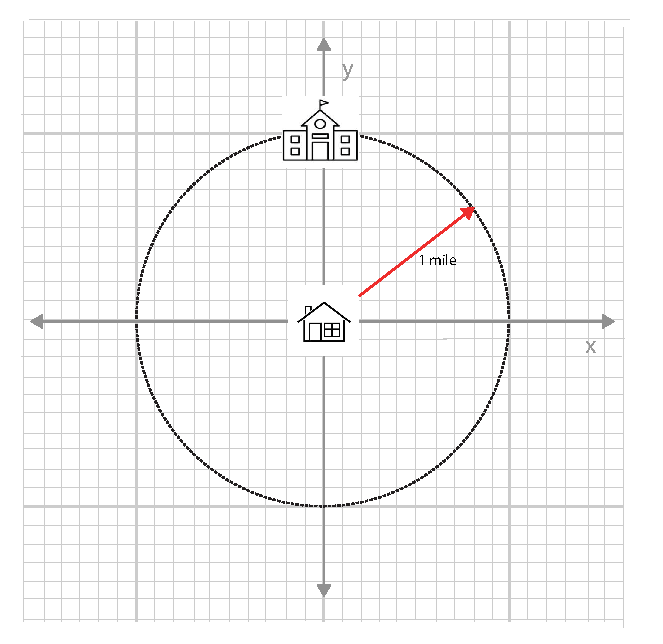
\includegraphics[scale = 0.7]{rect-vec.eps}
    \caption{Caption}
    \label{fig:rect-vec}
\end{figure}

Similarly the coordinates of the red vector are (8, 6) and we can write this as 8$\hat{x}$ + 6$\hat{y}$ miles. 

Hence, we are describing the vectors as a sum of an x-directed vector $\hat{x}$ and a y-directed vector $\hat{y}$. This can be written as $x \hat{x} + y\hat{y}$ where $x$ and $y$ are the x and y components of the vector respectively. 

%Here, the magnitude of the distance remains unchanged if we consider one big box (marked by a slightly bolder grey line on the grid) as one mile. As for the direction, we see that the school is on the y-axis. So, the position of the school can be written as 1 $\hat{y}$ mile. I will explain the meaning of $\hat{y}$ shortly; for now, just believe me that it means that the vector is magnitude 1 in y-axis.
There are some other ways of describing vectors as well, which we will explore in the last section. In the meantime, let's briefly see all the wonders we can do with vectors!

\section{Further Insights Into Vectors}
\subsection{Unit Vector}
We have just seen what magnitude is -- in simple words, it shows us how long a segment is. As you may have noticed, we used some letters with a "hat" to name the vectors of the previous examples (such as $\hat{x}$ and $\hat{y}$). And no -- we did not put them in that way for nothing! It is a special notation for \textbf{unit vectors}.

A unit vector, as its name states, has a \textbf{magnitude of 1}. That's the only requirement! This type of vector is usually denoted with a lowercase letter with a "hat", just like this:
%put an image with a unit vector and an a-hat

For example, v = (-3/5, 4/5) is a unit vector because: 

|v| = |(-3,5, 4/5)| = $\sqrt{(-3/5)^2 + (4/5)^2} = \sqrt{(9/25) + (16/25)} = \sqrt{25/25} = \sqrt{1} = 1$

{
\begin{center}
\fcolorbox{black}{shadecolor}{%

    \parbox{\textwidth}
    {%
        \small
        {
            \textbf{Fun Fact}:
            
            When you have a vector with the coordinates (0,0) it is called a \textit{zero vector}.
        }
    }%
}
\end{center}
}

\subsection{Conversion of Vector Representation}
As we mentioned before, vectors can be represented in diverse ways. In Fig. \ref{fig:polar} we explained polar representation; and on Fig. \ref{fig:rect-vec}, rectangular representation. 

On a not-so-random side note --could you imagine understanding a foreign language that you have never heard before \textit{without} a translator? Probably not. You would have to learn the brand new language to understand it by yourself. The very same things happens with different notations: sometimes, to understand them, we need to \textit{translate} them! Because of this, it is of utmost importance for you to know how to convert a vector from its polar form to its rectangular form and vice versa.

Here is an example: 
%put image of the example

Imagine you have a vector (2,2). This is written in its rectangular representation. However, if you observe really closely, you can realize that the diagram actually forms a right angle. This is \textbf{key} to know how to find the magnitude of the hypotenuse (in other words, the vector): the Pythagorean Theorem!

{
\begin{center}
\fcolorbox{black}{shadecolor}{%

    \parbox{\textwidth}
    {%
        \small
        {
            \textit{Side Note}: 
            The Pythagorean Theorem is a geometric theorem that uses the sum of the squares of both legs of the triangle to calculate the square of its hypotenuse. To put it in a simpler way, it follows the following formula: \[a^2 + b^2 = c^2\].
        }
    }%
}
\end{center}
}

If we apply the formula to our example, we would have the following mathematical calculations:

\begin{align*}
  2^2 + 2^2 &= c^2\\
  8 &= c^2\\
  \sqrt{8} &= c
\end{align*}

We now know that our hypotenuse's value is $\sqrt{8}$. As for the \textbf{angle}, we can find that using trigonometry. Since we know the three sides of the triangle, we can choose any trigonometric function we are most comfortable with. For this example, we will use \[\tan\theta = \frac{\text{opposite}}{\text{adjacent}}\]

So, for the tangent of this angle, it's \[\frac{2}{2} = 1\]

All we need to do now is take the inverse of that to have a final answer:

\[\theta = \tan^{-1}(1)\]
\[\theta = 45 ^{\circ}\]

\textbf{Congratulations!} You have now converted the vector's rectangular form into its polar form. The equality is as follows:

(2,2) = $\sqrt{8} \angle 45°$

And... \textit{what if we want to go the other way around? What if I want to convert a polar representation to a rectangular representation?}. That is a matter of simple trigonometry as well! 

%add image

To understand this, another brief example is this vector with magnitude r and an angle $\theta$. The \textbf{x coordinate} is \[r \cos\theta\] and the \textbf{y coordinate} is \[r \sin \theta\]. Thus, we can take some formulas to make the conversion process much faster:
\[r \angle \theta = (r \sin \theta, r \cos \theta)\]

Pretty simple, right? If there are any problems with the complex calculations (or short time), remember calculators are always there to help!

We are now masters of converting polar to rectangular forms but, how do we \textit{normally} operate with vectors? This topic will be discussed in the next section.

\section{Operations on Vectors}
With the extension of elementary algebra to vectors, we can now introduce \textbf{vector operations}.
\subsection{Addition}
Let's first consider vector $\overrightarrow{v}$ and  $\overrightarrow{w}$.
%draw both vectors with the tip-to-tail or parallelogram method

$\overrightarrow{v}$ + $\overrightarrow{w}$ is defined to be the resultant vector that goes from the tail of $v$ to the head of $w$. 
%drawing that pictures the sum
\subsection{Subtraction}
Another fun fact! Some mathematicians think that subtraction \textbf{does not exist}. Instead, it's just the inverse operation of addition. Thus, if we want to subtract $\overrightarrow{v}$ - $\overrightarrow{w}$, it could also be denoted as $\overrightarrow{v}$ + ($\overrightarrow{-w}$). With this concept, we can infer that the addition and subtraction of vectors are the same process -- just with a little \textit{twist}. The only difference is that we have to change the direction of the vector we are subtracting (in this case, $\overrightarrow{w}$). 
%put drawing 

\subsection{Scaling}
Before getting right into vector multiplication, we must first remember the unit vector. Why might this be useful? Well, vectors can be "scaled" off the unit vector. For example, vector a is shown to be 2,5 times a unit vector. 
%put image

\subsection{Multiplication}
Expanding more on scaling, this process is solely based on scalar multiplication. As you could see, a scalar multiplier k$>$0 can change the magnitude of the vector but not its direction. If k $<$ 0, then the scalar product will "reverse" the direction by 180 degrees.

For example, in rectangular form, if k is a scalar then
\[k(a,b) = (ka, kb)\]

\section{More Ways of Describing Vectors}
\subsection{Matrix Notation}
If you want to take your knowledge to the next level on vector notation, this is the right place to start! 

Matrices are defined as a rectangular array of numbers arranged in \textit{rows} and \textit{columns}. These numbers are called \textbf{elements}. Thus, the dimension of the matrix below is 2 x 3, since there are two rows and three columns:
%put any 2 x 3 matrix

{
\begin{center}
\fcolorbox{black}{shadecolor}{%

    \parbox{\textwidth}
    {%
        \small
        {
            \textit{Fun fact}: 
            Matrices are widely applied in engineering, economics, and statistics as well as in many other fields of mathematics! 
        }
    }%
}
\end{center}
}

A matrix with a single row is called a \textit{row vector} and a matrix with a single column is called a \textit{column vector}. The elements in a matrix are usually represented by lower case letters with a single subscript (e.g., \[a_j, b_j, x_j\]). Some examples of both types of vectors are shown below:

3 x 1 column vector: \[v = [y_1, y_2, y_3]\]
1 x 4 row vector: \[w = [h_1 h_2 h_3 h_4]\]
\subsubsection{Basic Concepts of Matrices}
In addition to those concepts, here are other basic terms that any good mathematician must know! 
A \textbf{square matrix} has the exact same number of rows and columns. 
%put example

A \textbf{diagonal matrix} is a square matrix where the \textit{diagonal elements} (elements where the two subscripts are equal) are nonzero and the \textit{off-diagonal elements} are zero.
%put example

The \textbf{identity matrix} is a type of diagonal matrix where every single diagonal elements are equal to 1. This particular matrix is usually represented as I. 
%put example

A \textbf{symmetric matrix} is a square matrix where the jk\textsuperscript{th} element is equal to the kj\textsuperscript{th} element.
%put example of 3x3 matrix --> M = [14,5,2//5,20,8//2,8,11]

Last but definitely not least, a \textbf{one vector} is a row or column vector in which every element is equal to 1.
%example --> 1 = [1 1 1]
\subsubsection{Matrix Operations}
\subsubsection{Addition}
The first thing you must check when adding a pair of matrices is their order. \textbf{Both must have an identical order!} For example, if you have two matrices (A and B) of order 2x2, then their sum would be as follows:
%put example

\subsubsection{Subtraction}
Similarly to vectors, we can apply the concept of "subtraction as the opposite of addition", meaning that A - B = A + (-B). Specifically, we would have to subtract each element of one matrix from the corresponding element of the second matrix. An example that depicts this is the following:
%put example

\subsubsection{Scalar Multiplication}
If you want to multiply a scalar by a matrix, you have to multiply the scalar number by every element on the matrix. 
%put example

\subsubsection{Matrix Multiplication}
Multiplying matrices has just one requirement: the number of columns of the first matrix must be equal to the number of rows in the second matrix. To understand this better, here we have an example:
%put example

\subsubsection{Dot Product}
Imagine that you have a solar panel (we love sustainable energy sources!). As the sun moves through the sky, the angle between sunlight and the solar panel changes.
%put two images: one with the sun at a 90 degree angle w the solar panel and another paralleled placed to it (explained below)

As we can see in the image, it would be ideal if the sun hit the solar panel at a 90° angle so it could capture the most energy possible. On the other hand, if the sunlight is placed paralleled to the panel, then it could not get any significant energy from this source. With this case, we can conclude that \textbf{the angle between a pair of objects is important.}
 When this is the case, we have the dot product to help us out.
 
 The \textbf{dot product} is an operation on vectors that enables us to easily find the angle between two vectors. To make this calculation, it is important to note that when we talk about the angle between two vectors, we're picturing the vectors with \textit{their tails at the same point.}
 %put image of "two vectors" and the "angle between them"
 
To depict this definition in more detail, here we have an example:

If we have vectors v = (1,2,3) and w = (4,5,6); then v*w = (1)(4) + (2)(5) + (3)(6) = 32

As we can see, the dot product is an operation between two vectors that produces a \textbf{scalar}. And to turn this into degrees, there's a key property of the dot product:

\textit{If $\theta$ is the angle between v and w, then $v*w = |\abs{a}||\abs{b}| \cos\theta$} (Remember that ∥a∥ represents the length of a!)
 
Using this information, we can now find the angle between v and w. By the Pythagorean Theorem,
\[∥v∥ = \sqrt{1^2 + 2^2 + 3^2} = \sqrt{14}\]
\[∥w∥ = \sqrt{4^2 + 5^2 + 6^2} = \sqrt{77}\]

So, 
\[32 = (\sqrt{14})(\sqrt{77})cos \theta\]

Therefore,
\[cos \theta = \frac{32}{(\sqrt{14})(\sqrt{77})} = \frac{32}{7\sqrt{22}}\]

So,
\[\theta = arccos(\frac{32}{7\sqrt{22}})\]

\subsection{Dirac Notation}
Being, also called bra-ket notation, dirac notation used the angle brackets ($\langle$ and $\rangle$) and a vertical bar (|) to construct "bras" and "kets".

A \textbf{ket} denotes a vector in an abstract vector space. If we are talking in physical terms, kets also represent a state of a quantum system. A ket looks like this: "{$\displaystyle |v\rangle$ }" A common example is:
\[|\psi \rangle = \]

A \textbf{bra}, in short, denotes a linear form 
\chapter{Introduction to Python}
\label{ch:python}

\begin{center}
\fcolorbox{black}{shadecolor}{%

    \parbox{\textwidth}
    {%
        \small
        {
            This chapter is a basic introduction to programming in Python. If you have previous experience, feel free to proceed to the next chapter.
        }
    }%
}
\end{center}

\section{So, What is Python?}
Python, a programming language globally known for its straightforward syntax, is now one of the most popular languages between developers. And by learning how to master it, you can become one too!

Writing programs is a truly rewarding (and creative) activity. You can have diverse reasons to write a program, varying from solving a difficult data analysis to having genuine fun. Regardless if you like math or not, you do not have to be a great mathematician to be an awesome programmer. 
Even though this chapter is not necessarily intended for professional programmers, advanced programming can be really rewarding (and for the sake of ZX Calculus, it's completely necessary!)

In short you need two main skills to be a programmer:
\begin{itemize}
    \item Know the programming language (Python), including the vocabulary and the grammar. It's like mastering an actual language! You must be able to construct well-formed "sentences".
    \item Tell a story. And by this I mean that you have to combine words and sentences to convey an idea to the reader. In this case, our program is the "story" and the problem we are trying to solve is the "idea".
\end{itemize}

\section{Programming Platform Installation}
First things first. Before getting right into explaining Python's vocabulary, we will explain a simple way to actually start to code in Python. For this, we will use \textbf{Google Colaboratory}. There other ways to download Python but, for the sake of simplicity, we will use an online program. Follow these steps to create a Python file:

\begin{enumerate}
    \item Open Google Chrome and access your Gmail account. If you don't have one, please refer to \href{https://support.google.com/mail/answer/56256?hl=en}{this link} and follow the instructions.
    \item When your account is already set, click on the 9-dot-structure placed on the upper right section of your screen and open Drive. This has a triangle-like logo.
    \item Click on "New" to create a new document. Then, click on "More" and here you will find the option to "Connect more apps".
    \begin{figure}[H]
        \centering
        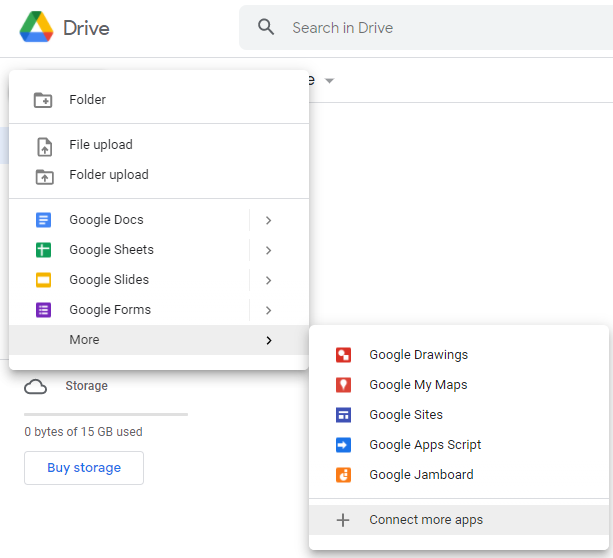
\includegraphics[width = 0.5\textwidth]{Screenshot(15).png}
        \caption{"Connect more apps" option}
        \label{fig:connect-more-apps}
    \end{figure}
    \item A "Google Marketplace Workplace" will appear. Type in the search box "Colaboratory".
    \begin{figure}
        \centering
        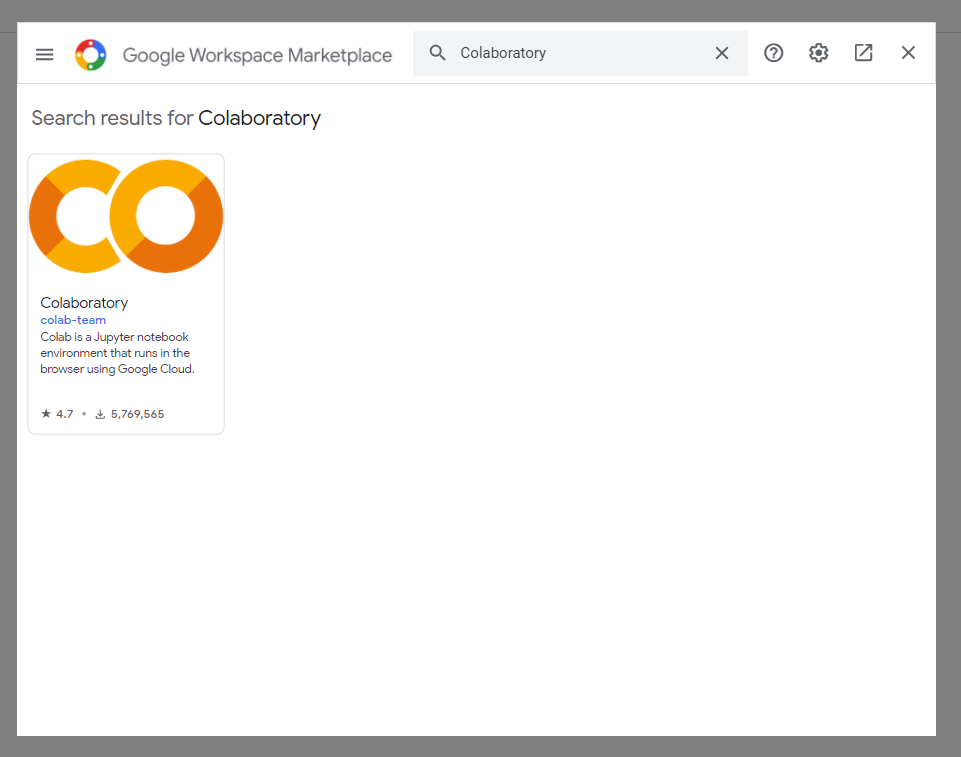
\includegraphics[width=0.5\textwidth]{Figures/Screenshot(18).png}
        \caption{"Google Marketplace Workplace" tab}
        \label{fig:search-colab}
    \end{figure}
    \item Install Google Colaboratory clicking in the blue "Install" button.
    \item To create a new document, press again the "New" button in Drive, then "More" and finally, "Google Colaboratory".
    \begin{figure}[htb]
        \centering
        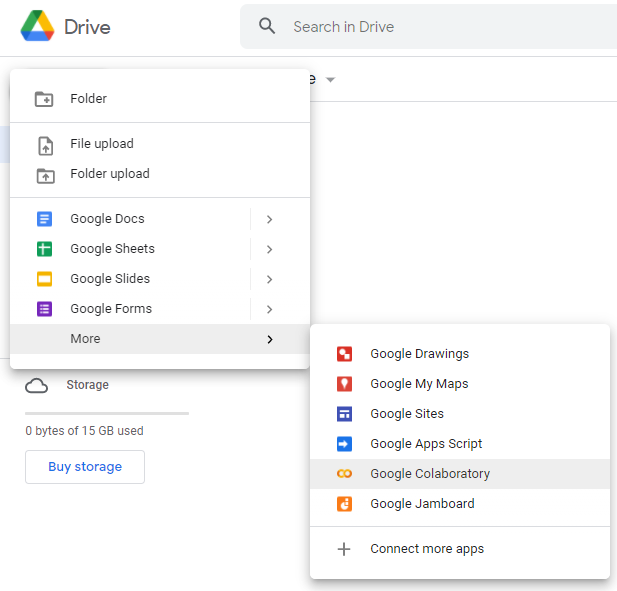
\includegraphics[width=0.5\textwidth]{Figures/Screenshot(21).png}
        \caption{"Google Marketplace Workplace" tab}
        \label{fig:google-marketplace}
    \end{figure}
    \item Congratulations! You have now created a Python file. All the changes you do from now on in the document are automatically saved (yay!).
\end{enumerate}

Now that we have that covered, let's start with the vocabulary and structure of Python programs.

\section{Words and Sentences: Hello, World!}
Imagine that you have a dog. When we want to train a dog, we normally use special words such as "sit", "walk" or "stop". If you talk to the dog and don't use the words you previously taught, they will simply not understand you. For example, if you say, "I wish I could just walk to my best friend's house to play Roblox", what your dog would hear is, "blah blah blah \textit{walk} blah blah blah." 

Similarly, there are words that have a very special meaning to Python. When Python sees these specific words in a program, they have one \textbf{and only one} meaning to Python. Later on, you will also be able to create words with unique meanings on their own called \textit{variables}. In these, you will be able to choose your names for your variables, but this is nothing of the sort with Python's reserved words. 

These reserved words are the following:

\begin{minipage}{\linewidth}
    \begin{spverbatim}
      and, as, assert, break, class, continue, def, del, elif, else, except, finally, for, from, global, if, import, in, is, lambda, nonlocal, not, or, pass, raise, return, try, while, with, yield
    \end{spverbatim}
\end{minipage}

And that's it! The best part is that (unlike a dog) Python is already trained. 

We will learn these reserved words and how they are used in a while, but for now we will focus on the Python equivalent of “speak”. The nice thing about telling Python to speak is that we can even tell it what to say by giving it a message in quotes:

\begin{minted}{python}
print("Hello, World!")
\end{minted}

Our sentence starts with the function print followed by a string of text of our choosing enclosed in single quotes. Try to type it in your Google Colaboratory document! When you have it ready in the cell, click the arrow at the left and you should have the following output:
 \begin{minted}{python}
>>> print("Hello, World!")
Hello, World!
 \end{minted}

You can also print numbers, like this!
\begin{minted}{python}
>>> print(1)
1
\end{minted}

\section{The building blocks of programs}
There are some conceptual patterns that we use to construct programs or, in other words, \textbf{algorithms}. These basic concepts are the following:

\textbf{input} Get data form the user. In our first programs, our input will come from the user typing data on the keyboard.

\textbf{output} Display the results of the program on a screen or store them in a file.

\textbf{sequential execution} Perform statements one after another in the order they are encountered in the program.

\textbf{conditional execution} Check for certain conditions and then execute or skip a sequence of statements.

\textbf{repeated execution} Perform some set of statements repeatedly, usually with some minor variation.

\section{Variables, expressions, and statements}
\subsection{Values and types}
A \textit{value} is a basic component a program works with, such as a letter or a number. The only values we have learned so far are 1 and "Hello, World!"

These values have different \textit{types}: 1 is an integer, and "Hello, World!" is a string (it's called that way because it contains a "string" of letters. These are \textbf{always} enclosed in quotation marks).

If you are not sure what type a value has, you can always receive help from the interpreter:
\begin{minted}{python}
>>> type("Hello, World!")
<class 'str'>

>>> type(43)
<class 'int'>

\end{minted}

There's also another type of value called \texttt{float}, which belongs to numbers with a decimal point.
\begin{minted}{python}
>>> type(5.9)
<class 'float'>
\end{minted}

If numbers are between quotation marks, they are considered strings.
\begin{minted}{python}
>>> type('43')
<class 'str'>
    
>>> type('5.9')
<class 'str'>  
\end{minted}

\subsection{Variables}
One of the most powerful features of a programming language is the ability to manipulate \textit{variables}. A variable is a name that refers to a value. To do this, you just have to assign a value to a variable. A few examples are:
\begin{minted}{python}
>>> greeting = "Hello, my friend!"
>>> age = 16
>>> pi_value = 3.1415926535897931

\end{minted}
This example makes three assignments. The first assigns a string to a new variable named \texttt{greeting}; the second assigns the integer 16 to \texttt{age}; the third assigns the approximate value of pi to $pi_value$.

These values can also be displayed as follows:

\begin{minted}{python}
>>> print(age)
16
    
>>> print(pi_value)
3.1415926535897931
\end{minted}

The type of a variable is the type of the value it refers to.

\begin{minted}{python}
>>> type(greetings)
<class 'str'>
    
>>> type(age)
<class 'int'>
    
>>> type(pi_value)
<class 'float'>
\end{minted}

\subsection{Variable names and keywords}
Variable names can be as long as you want it to be. They can contain both letters and numbers; still, they cannot start with a number. You \textit{can} use uppercase letters to name variables, but it's better to begin with lowercase letters (don't worry, you'll get this later). 
Underscores $(_)$ are often used in multiple-word variables, such as $my_name$.

It is of utmost importance to note that by ANY circumstance, you \textbf{cannot} use a Python keyword as a variable (e.g. class = "Maria's party"). The interpreter uses keywords to recognize the structure of the program, hence they cannot be used as variable names.

Python has 35 keywords:

\begin{minipage}{\linewidth}
    \begin{spverbatim}
        and, as, assert, break, class, continue, def, del, elif, else, except, False, finally, for, from, global, if, import, in, is, lambda, None, nonlocal, not, or, pass, raise, return, True, try, while, with, yield, async, await
    \end{spverbatim}
\end{minipage}

Be sure to take this into account when you create variables!

\subsection{Statements}
A \textit{statement} is defined as a unit of code that the Python interpreter can execute. A program usually contains a sequence of statements. If there is more than one statement, the results appear one at a time as the statements execute. For example:
\begin{minted}{python}
print(1)
x = 2
print(x)
\end{minted}

has the output of:
\begin{minted}{python}
1
2
\end{minted}

\subsection{Operators and Operands}
I know we already said that you don't have to be a great mathematician to be an awesome programmer, but it can definitely help you improve! For this, we have operators. \textit{Operators} are special symbols that represent computations like addition and multiplication. The values the operator is applied to are called \textit{operands}.

The operators \texttt{+}, \texttt{-}, \texttt{*}, \texttt{/}, and \texttt{**} perform addition, subtraction, multiplication, division, and exponentiation respectively. For example:
\begin{minted}{python}
25 + 34
55-35
5*3
10/2
5**2
\end{minted}

The division symbol we see above gives us a \texttt{float} (meaning that the result will be in decimal form). In addition to this, we also have the integer division, in which we will use two slashes \texttt{(//)}.
\begin{minted}{python}
>>> x = 40
>>> x//5
8
\end{minted}

\subsection{Expressions}
An \textit{expression} is a combination of values, variables, and operators. A value all by itself is considered an expression, and so is a variable. Here we have 3 brief examples:
\begin{minted}{python}
    17
    x
    x + 17
\end{minted}

Remember that, in a script, an expression all by itself doesn’t do anything! This is a common
source of confusion for beginners. This can be seen in the example above, as \texttt{17} is not printed. Instead, the result of \texttt{x + 17} can be seen. Try it out in Google Colaboratory!

Another detail we must mention is the \textit{rules of precedence}. You can use acronyms (such as PEMDAS) to remember the rules:
\begin{enumerate}
    \item Parentheses ()
    \item Exponentiation (x**y)
    \item Multiplication and Division (* and / or //)
    \item Addition and Subtraction (+ and -) in order of precedence from left to right
\end{enumerate}

\subsection{String operations}
The \texttt{+} operator works with strings, but it is not addition in the mathematical sense. Instead, it performs \textit{concatenation}, which means joining the strings. For example:
\begin{minted}{python}
>>> a = '100'
>>> b = '200'
>>> print(a+b)
100200
\end{minted}

The \texttt{*} operator also works with strings by multiplying the content of a string by an integer. For example:
\begin{minted}{python}
>>> a = 'Hello '
>>> b = 3
>>> print(a * b)
Hello Hello Hello
\end{minted}

\subsection{Asking the user for input}
If you want to make a "personalized" program by taking the input of the user via the keyboard, there is a way to do so! Python provides a built-in function called \texttt{input} that gets input from the keyboard. When this function is called, the program stops and waits for the user to type something. When the user presses Enter, the program resumes and input returns what the user typed as a string.
\begin{minted}{python}
>>> name = input("What is your name?\n")
Maria
>>> print(name)
Maria
\end{minted}

The sequence at the end of the prompt represents a newline, which is a special character that causes a line break.

\subsection{Comments}
As your program turns out to be more and more complex, you sometimes need to remember some things so you can read it efficiently. Because of this, it is a good idea to add notes into your programs to explain in natural language what a statement/expression is doing. These are \textit{comments}, and in Python we can add them with the hashtag symbol.
\begin{minted}{python}
#find how many seconds are in a specific number of minutes
seconds = minute * 60
\end{minted}

These do not affect your code, so you can write anything you want!

\section{Conditionals}
\subsection{Boolean expressions}
A \textit{boolean expression} is an expression that is either true or false. For this, we use the operator ==, which compares two operands and produces True if they are equal and False otherwise:
\begin{minted}{python}
>>> 5 == 5
True
    
>>> 5 == 10
False
\end{minted}

It is like we are asking to Python, "Are x and y equal?". Remember that one equal symbol (=) is solely for assigning variables.

\texttt{True} and \texttt{False} are special values that belong to the class bool; they are not strings:
\begin{minted}{python}
>>> type(True)
<class 'bool'>

>>> type(False)
<class 'bool'>

\end{minted}

== is only one of all the \textit{comparison operators}. The rest are:
\begin{minted}{python}
    x > y          #x is greater than y
    x < y          #x is less than y
    x >= y         #x is greater than or equal to y
    x <= y         #x is less than or equal to y
    x != y         #x is not equal to y
    x is y         #x is the same as y
    x is not y     #x is not the same as y
\end{minted}

\subsection{Logical operators}
There are three \textit{logical operators}: \texttt{and}, \texttt{or} and \texttt{not}. The meaning of each one is actually straightforward (really similar to their meanings in English). For example:
\begin{minted}{python}
x > 0 and x < 5
\end{minted}
is ONLY true if x is greater than 0 \textit{and} less than 5.

Another example:
\begin{minted}{python}
n%2 == 0 or n%3 == 0
\end{minted}
is true if \textit{either} of the conditions is true (in other words, if n is divisible by 2 \textit{or} 3).

Finally, the \texttt{not} operator negates a boolean expression. Thus:
\begin{minted}{python}
not (x > y)
\end{minted}
is true if x > y is \textit{false} (in other words, if x is less than or equal to y).

\subsection{Conditional execution}
To write useful and effective algorithms, we almost always (if not always) need to include conditions that change how the program is executed according to the circumstances. Because of this is reason is that we use \textit{conditional statements}. The simplest of these is the \texttt{if} statement:
\begin{minted}{python}
if x < 5:
    print("x is lower than 5") #condition
\end{minted}

As you could see in the comment, the boolean expression after the \texttt{if} statement is called a \textit{condition}. For the if statement to have a correct syntax, we must put a colon (:) to end the statement, and the line(s) after the statement must be indented. 

\texttt{if} statements have the same structure as for loops (we will learn about them moreover). Both of these are categorized as \textit{compound statements}, since they are longer than a single code line. 

\section{Alternative execution (if, else)}
We also have the option to specify an \textit{alternative execution}. This means, in English, that "if this statement is \texttt{False}, then we can do this other statement" instead of just passing it off. The syntax would look like the following:
\begin{minted}{python}
if x%3 == 0:
    print("x is divisible by 3")
else:
    print("x is not divisible by 3")
    
\end{minted}
If the remainder when x is divided by 3 is 0, then we know that x is divisible by 3, and the program displays a message to that effect. If the condition is \texttt{False}, the second set of statements is executed.

\subsection{Chained conditionals (if, elif, else)}
Thought only one alternative was not enough? Sometimes, we there are more than two possibilities! \textit{Chained conditionals} allows us to do this.
\begin{minted}{python}
if x < y:
    print("x is less than y")
elif x > y:
    print("x is greater than y")
else:
    print("x and y are equal")
\end{minted}
Fun Fact! \texttt{elif} is an abreviation of "else if". The best part of this is that there are \textbf{no} limit on the number of \texttt{elif} statements we can add. Also, it's not necessary to add an \texttt{else} clause. The only requirement is that it must be at the end but if you don't want it there, o pressure at all!

\begin{center}
\fcolorbox{black}{shadecolor}{%

    \parbox{\textwidth}
    {%
        \small
        {
            \textit{Friendly reminder:}
            Every condition is checked in order. If the first is false, the next is checked, and so on.
        }
    }%
}
\end{center}

\subsection{Nested conditionals}
Level up! One conditional can \textbf{also} be nested within another (surprise!). Thus,
\begin{minted}{python}
if x == y:
    print("x and y are equal")
else:
    if x < y:
        print("x is less than y")
    else:
        print("x is greater than y")
\end{minted}
They are pretty confusing sometimes, so it is recommended to avoid them when you can. 

\section{Functions}
\subsection{Function calls}
A \textit{function} is a named sequence of statements that performs a computation. For example:
\begin{minted}{python}
>>> type(32)
<class 'int'>
\end{minted}
The name of the function is \texttt{type}. The expression in parenthesis is called the \textit{argument} of the function, and the result, for the type function, is the type of argument.

Sometimes, you may hear that the function "takes" an argument and "returns" a result. The result is called the \textit{return value}.

\subsection{Built-in functions}
As it name states, there are some functions that we can use without needing to provide the function definition. These are:
\begin{minted}{python}
>>> max("Hello, World!")
"w"
    
>>> min("Hello, World!")
" "
\end{minted}
The max function tells us the “largest character” in the string (which turns out to be the letter “w”) and the min function shows us the smallest character (which turns out to be a space).

Another very common built-in function is the \texttt{len} function which tells us how many
items are in its argument. If the argument to \texttt{len} is a string, it returns the number of characters in the string.
\begin{minted}{python}
>>> len("Hello, World!")
13
\end{minted}

\subsection{Type conversion functions}
In some specific circumstances, you need to convert values from one type to another. We can do this with built-in functions. 

You can use the \texttt{int} function to convert a float value to an integer.
\begin{minted}{python}
>>> int('32')
32
\end{minted}
When converting an \texttt{int} into a \texttt{float}, it doesn't round it off. Instead, it chops off the fraction part. 
\begin{minted}{python}
>>> int('5.998')
5
\end{minted}
\texttt{float} can convert integers and strings:
\begin{minted}{python}
>>> float(32)
32.0
\end{minted}
Last but not least, \texttt{str} converts its argument to a string:
\begin{minted}{python}
>>> str(32)
'32'
\end{minted}

\subsection{Math functions}
In case someone wants to work with mathematical functions, Python has a \texttt{math} module that provides most of the familiar ones. To use it, we first have to import it:
\begin{minted}{python}
>>> import math
\end{minted}

With this, we created a module object named math. This module object contains the functions and variables defined in the module. To use one of these functions, you must specify the name of the module and the name of the function. Remember to separate these with a dot! 
\begin{minted}{python}
>>> ratio = signal_power / noise_power
>>> decibels = 10 * math.log10(ratio)

>>> radians = 0.7
>>> height = math/sin(radians)
\end{minted}

This first example computes the logarithm base 10 of the signal-to-noise ratio. On the other hand, the second example finds the sine of \texttt{radians}. The conversion of degrees to radians is made first dividing the value by 360 and multiplying it by $2\pi$.
\begin{minted}{python}
>>> degrees = 45
>>> radians = degrees / 360.0 * 2 * math.pi
>>> math.sin(radians)
0.7071067811865476
\end{minted}

In the previous code, the expression \texttt{math.pi} gets the variable \texttt{pi} from the math module.

\subsection{Random numbers}
The \texttt{random} module provides functions that generate pseudorandom numbers (or, in short, "random" numbers).
\begin{minted}{python}
import random

for i in range(10):
    x = random.random()
    print(x)
\end{minted}
This would produce 10 random numbers between 0.0 and up to (but NOT including) 1.0.
\begin{minted}{python}
0.11132867921152356
0.5950949227890241
0.04820265884996877
0.841003109276478
0.997914947094958
0.04842330803368111
0.7416295948208405
0.510535245390327
0.27447040171978143
0.028511805472785867
\end{minted}

\subsection{Adding new functions (def)}
Python also let's your creativity develop! It is also possible to add new functions. A \textit{function definition} defines the name of a brand new function and the sequence of statements that must be executed when the function is called. Here is an example:
\begin{minted}{python}
def printsonglyrics():
    print("I see a little silhouetto of a man")
    print("Scaramouch, Scaramouch, will you do the Fandango!")
\end{minted}
\texttt{def} is a keyword that indicates that this is a function definition. The function, in this case, is \texttt{printsonglyrics}. The empty parenthesis after the name indicate that the function doesn't take any arguments. 

\subsection{Why functions?}
But after all of this explanation, why do we use functions? There are several reasons:
\begin{itemize}
    \item You can name a group of statements, which makes your code shorter and easier to read.
    \item You eliminate repetitive code! The smaller your code is, the better.
    \item Once you write a well-designed function, you can reuse it.
\end{itemize}

\section{Iteration}
\subsection{Updating variables}
A common practice in the world of programming is the use of an assignment statement that updates a variable.
\begin{minted}{python}
x = x + 1
\end{minted}

This means that the final updated value of x will be "the previous value of x added by 1". But before you try to update a variable, you need to initialize it. Like this, for example:
\begin{minted}{python}
>>> x = 0
>>> x = x + 1
\end{minted}

\subsection{The \texttt{while} statement}
Computers are really (really!) good at repeating identical tasks without making errors. To do this, Python provides several features to make this programming process easier. A clear example is the \texttt{while} statement. Here is a simple program to portray what it does:
\begin{minted}{python}
n = 3
while n > 0:
    print(n)
    n = n -1
print("Fire!")
\end{minted}

More formally, the \texttt{while} statement does te following:
\begin{enumerate}
    \item Evaluate the condition (Is it \texttt{True} or \texttt{False}?)
    \item If the condition is false, exit the \texttt{while} statement and continue execution at the next statement.
    \item If the condition is true, execute the body and go back to step 1. 
\end{enumerate}

This makes us introduce a really important concept: a \textit{loop}. Each time we execute the body of the loop is called an \textit{iteration}. Thus, for the above loop, we would say that "It had 3 iterations". 

The body of the loop should change the value of one or more variables so that eventually the condition becomes false and the loop terminates. If this doesn't happen, the loop will repeat forever, resulting in an \textit{infinite loop}.

\subsection{Definite \texttt{for} loops}
Imagine that you have a list. Sometimes, we want to loop through a set of things, and when this is the case, we use a \textit{definite} loop using a \texttt{for} statement. We call the \texttt{while} statement an \textit{indefinite loop} because it simply loops until some condition becomes \texttt{False}. However, the \texttt{for} loop is looping through a known amount of items. Because of this, it runs as many iterations as there are items. Here is an example:
\begin{minted} {python}
friends = ["Rafaela", "Lucia", "Jose"]
for friend in friends:
    print("Happy New Year:", friend)
print("Done!")
\end{minted}

The output would be:
\begin{minted}{python}
Happy New Year: Rafaela
Happy New Year: Lucia
Happy New Year: Jose
Done!
\end{minted}

The \texttt{for} loop is going through the list and executes the body once for each of the three strings of the list.

\section{Strings}
\subsection{What is a string?}
A string is a \textit{sequence} of characters. You can access the characters one at a time with brackets:
\begin{minted}{python}
>>> fruit = "banana"
>>> letter = fruit[1]
\end{minted}

With this, we are extracting the character at index position 1 from the \texttt{fruit} variable and assigns it to the \texttt{letter} variable. The output of the code above is:
\begin{minted}{python}
>>> print(letter)
a
\end{minted}

What? Isn't the first letter of "banana", "b"? In Python, the index is an offset from the beginning of the string, and the offset of the first letter is zero.
\begin{minted}{python}
>>> letter = fruit[0]
>>> print(letter)
b
\end{minted}

"b" is the 0th letter of "banana", while "a" is the 1th letter. 

\subsection{Length of a string (len)}
\texttt{len} is another built-in function that returns the number of characters in a string.
\begin{minted}{python}
>>> fruit = "banana"
>>> len(fruit)
6
\end{minted}

It's really that straightforward! Anoher way you can use this is with negative indices.
\begin{minted}{python}
>>> fruit = "banana"
>>> last = fruit[-1]
>>> print(last)
a
\end{minted}

The expression \texttt{fruit[-1]} denotes the last letter; \texttt{fruit[-2]}, the second to last, and so on.

\subsection{Slicing strings}
As it's name depicts, slicing strings is the act of dividing a string into segments. For example:
\begin{minted}{python}
>>> a = "Maria Fernanda"
>>> print(a[0:5])
Maria
\end{minted}

The operator returns the part of the string from the "n-th" character to the "m-th" character, including the first but excluding the last.

There are also other ways to make the operator even more brief. We can do this using colons. 
\begin{minted}{python}
>>> fruit = "banana"
>>> fruit[:3]
"ban"

>>> fruit[3:]
"ana"
\end{minted}

The colon (:) allude to all the characters before the third one, without including the third one in the first example. The second one uses the same methodology, but with all the last characters from 3 onward. 

\subsection{The \texttt{in} operator}
\texttt{in} is a boolean operator that takes two strings and returns \texttt{True} if the value appears in the string. For example:
\begin{minted}{python}
>>> "a" in "banana"
True

>>> "z" in "banana"
False
\end{minted}

\subsection{String comparison (==)}
To see if two strings are equal, we can use a double equal sign. Like this!
\begin{minted}{python}
if word == "hello"
    print("Hello, my friend!")
\end{minted}

You can also use comparison operators to put strings in alphabetical order:
\begin{minted}{python}
if word < "hello":
    print("Your word, " + word + ", comes before hello.")
elif word > "hello":
    print("Your word, " + word + ", comes after hello.")
else:
    print("Hello, my friend!")
\end{minted}

\section{Lists}
\subsection{What is a list?}
A \textit{list} is a sequence of values. In a string, the values are characters but, in a list, they can be any type. The values in a list are called \textit{elements}. To do a list, you just have to encose the elements in square brackets.
\begin{minted}{python}
[5, 10, 15, 20, 25]
["air", "fire", "water", "earth"]
\end{minted}

The first example is a list of five integers. The second is a list of four strings. You can also \textit{nest} a list within another, like this:
\begin{minted}{python}
["hello", 5.2, 6, [3, 6]]
\end{minted}

Similarly to strings, you can also assign lists a variable:
\begin{minted}{python}
>>> food = ["Hamburger", "Pizza", "Spaghetti"]
>>> ages = ["11, 16, 18, 21]
>>> empty = []
>>> print(food, ages, empty)
["Hamburger", "Pizza", "Gouda"] [11, 16, 18, 21] []
\end{minted}

\subsection{List operations}
The \texttt{+} operator \textit{concatenates} (hope you remember the term!) lists:
\begin{minted}{python}
>>> a = [1, 2, 3]
>>> b = [4, 5, 6]
>>> c = a + b
>>> print(c)
[1, 2, 3, 4, 5, 6]
\end{minted}

The \texttt{*} operator repeats a list depending on the number:
\begin{minted}{python}
>>> [1] * 4
[1, 1, 1, 1]

>>> [4, 5, 6] * 3
[4, 5, 6, 4, 5, 6, 4, 5, 6]
\end{minted}

\section{Dictionaries}
You probably already know pretty well what a dictionary is. And the definition of a \textbf{Python} library is not that far fetched. A \textit{dictionary} is similar to a list, but a little bit more general. In a list, the index positions must be integers, but in a dictionary, indices can be any type (almost).

To give you an example, we will build a dictionary that maps from English to Spanish words, so the keys and the values are \textbf{strings}.

The function \texttt{dict} creates a new dictionary. 
\begin{minted}{python}
>>> dictionary_1 = dict()
>>> print(dictionary_1)
{}
\end{minted}

The curly brackets, \texttt{{}}, says that the dictionary is empty. To add elements to it, you can use square brackets like this:
\begin{minted}{python}
>>> dictionary_1["hello"] = "hola"
\end{minted}
This examples creates an item that maps from the key \texttt{"hello"} to the value \texttt{"uno"}.

\textit{Voila!} If we print the dictionary one more time, we can see a key-value pair with a colon between both:
\begin{minted}{python}
>>> print(dictionary_1)
{"hello" : "hola"}
\end{minted}

You can also add items to a dictionary in an input format. For example, you can create a new dictionary with three items. But if you print it, you might be surprised:
\begin{minted}{python}
>>> dictionary_1 = {"hello": "hola", "goodbye": "adiós", "morning": "mañana"}
>>> print(dictionary_1)
{"hello": "hola", "morning": "mañana", "goodbye": "adiós"}
\end{minted}

The order of the items of a dictionary is unpredictable. Because of this, the key-value pairs will not necessarily be the same. But no worries! It's not a problem at all.Since the elements of a dictionary are never indexed with integer indices, we can use the keys to look up the corresponding values:
\begin{minted}{python}
>>> print(dictionary_1["goodbye"])
"adiós"
\end{minted}

You can also use the \texttt{len} function to know the number of key-value pairs:
\begin{minted}{python}
>>> len(dictionary_1)
3
\end{minted}

\section{Your learning journey}
\textbf{You rock!} You finished the first chapter. We are really proud of you for pushing through! 

Don’t be afraid if the concepts don’t seem to fit together well the first time. We want you to learn Python much more rapidly, but it is like learning a new language that takes time to absorb and understand before it feels natural.By reviewing previous material and even doing some exercises, you will realize that you actually learned a lot of material even if it seems a bit impenetrable at first sight! 

Usually when you are learning your first programming language, there are a few wonderful “Ah hah!” moments where you realize you are making an amazing work.

If something seems particularly hard, there is usually no value in staying up all night and staring at it. \textbf{Take a break}, take a nap, have a snack, watch some Netflix, explain what you are having a problem with to someone (or perhaps your dog), and then come back to it with fresh eyes. I assure you that once you learn the programming concepts in the chapter, you will look back and see that it was all really easy and elegant and it simply took you a bit of time to absorb it.

Using Python is the backbone of quantum computing, so don't be afraid of trying over and over again. In the next chapters, you will immerse into the world of physics and how this strongly related to quantum computing and quantum mechanics. Remember: \textbf{take it slow}. You will get there eventually!

In the next section, you will find some exercises that wrap up everything you made in the chapter. Feel free to complete them to gain confidence about all the knowledge you acquired! If you have any questions about the resolution of one of the problems, do not hesitate to contact us. You can find our email in our website. Good luck and happy coding!

\section{Exercises}
Complete these questions to remember everything you learned in the chapter!

\textbf{Exercise 1.} Define a statement, an expression and a variable.

\textbf{Exercise 2.} Write a program that uses input to ask the user their name and greet them.
\begin{verbatim}
    Enter your name: Maria
    Hello, Maria!
\end{verbatim}

\textbf{Exercise 3.} Write a program that computes the following: If x is greater than z, then print "Congratulations! x is greater than z". If x is smaller than z, print "Try it another time! x is smaller than z". If x and z are equal, print "It's a tie!x and z are equal."

\textbf{Exercise 4.} What is the "def" keyword for in Python?
a) It indicates that the following indented section is to be stored for later use

b) It indicates the start of a new function

c) It is a slang that means "the following code is nice"

d) a and b are correct

e) None of the above

\textbf{Exercise 5.} What will be the output of the following Python program?
\begin{minted}{python}
def myname():
    print("Lucia")
def myfriend():
    print("Fernanda")

myfriend()
myname()
myfriend()
\end{minted}

a) Lucia Fernanda myfriend myname myfriend

b) Lucia Fernanda Lucia

c) Fernanda Lucia myfriend

d) Lucia Lucia Lucia

e) Fernanda Lucia Fernanda

\textbf{Exercise 6.} Write a program that reads numbers repeatedly until the user enters "done".
\begin{minted}{python}
Enter a number: 5
Enter a number: 45
Enter a number: hello
Invalid input. Please write a number.
Enter a number: 6
Enter a number: done
\end{minted}

\textbf{Exercise 7.} Imagine you have this string: s = "dshduyhddsnbobobskj". Find how many times "bob" is repeated using string slicing.

\textbf{Exercise 8.} It is a well known fact that Shakespeare used over 20,000 words in his works all in total. However, how could you determine that in code? Let's use Python for this! List all unique words, sorted in alphabetical order, that are stored in a file \texttt{romeo.txt} containing a subset of Shakespeare's work. To do this efficiently, download a copy of \href{www.py4e.com/code3/romeo.txt}{this file}.

\textbf{Exercise 9.} Why are functions used?

\textbf{Exercise 10.} What is a dictionary? Why are they important in Python?

\section{Further resources}
Do you want to deepen your knowledge in Python? Here we leave you some great sources you can follow. 

\begin{itemize}
    \item \href{https://www.learnpython.org/}{learnpython.org}
    \item \href{https://www.youtube.com/watch?v=Z1Yd7upQsXY&list=PLBZBJbE_rGRWeh5mIBhD-hhDwSEDxogDg}{CS Dojo}
    \item \href{https://www.youtube.com/watch?v=jjqgP9dpD1k&list=PL6beirVtPMMFDD_wzVb2g8CPfVrBuOAkI}{CS50}
    \item 
\end{itemize}
% \chapter{Diagrammatic Representation}
\chapter{ZX-Calculus: First Contact}

% \begin{lstlisting}[language = Python]
% import pyzx
% \end{lstlisting}

To study quantum computing, we have a few special-purpose notations:
\begin{itemize}[leftmargin = *]
    \item \textbf{Quantum Circuits:} This notation studies quantum computing on an implementation level. It explores the components required to build quantum circuits and their \textit{tuning} for optimal performance. This involves both designing and hardware implementation of quantum circuits.   
    \item \textbf{Measurement Calculus:} This notation entails a mathematical study of quantum circuits. Making use of mathematical tools, it studies the \textit{manipulation} of quantum data at different stages of quantum circuits. 
\end{itemize}

ZX-calculus falls in the second category of notations. It makes use of the complementarity of Z-basis and X-basis, and defines the quantum circuits in a graphical language so that they are more mathematically elaborate. The advantage is the understanding of quantum algorithms beyond gate-level implementation -- among many.

This chapter is dedicated as an introduction to the notation of ZX-Calculus and its elements. It will make use of PyZX, a Python package for ZX-Calculus, to provide an early acquaintance to this tool. PyZX itself will be explored in more detail in the next chapter.  

\section{PyZX: Python Library for ZX-Calculus}
As we mentioned in chapter \ref{ch:python}, programming is a tool used by engineers, scientists, and pretty much everyone for assistance in computation. We also introduced you to libraries with the promise that we will be using them often. In fact, we will be actively working with coding throughout this book.

PyZX (pronounced as `pixie') is a python library for assisting with the visualisation of ZX-calculus diagrammatics and for computationally optimising the ZX-graphs.

For installing PyZX, run the following command using either the terminal or your Jupyter notebook:
\begin{python}
pip install pyzx
\end{python}

Once installed, you can use PyZX in your Python program by importing it. For that, use: 

\begin{python}
import pyzx
\end{python}

We will not dive into PyZX any deeper in this chapter and will come back to it in chapter \ref{ch:pyzx} when we are in a better position of understanding ZX-Calculus and appreciating PyZX. For now, this much detail will suffice for our working.  

\section{Building Blocks}
The ZX-Calculus language is composed of several building blocks which connect together to form the diagrams. As the ZX-Calculus is a graphical diagramamtic language, it chiefly consists of nodes and edges. We will explain them one by one in this section:

\subsection{Wires}
You may have known about electric wires from the circuits in your home and from your science books; they are used to connect the components of an electrical circuit together. Very much like that, we have wires in ZX-Calculus language to connect different components together. However, do not think them of a carrier of electrons like in a classical electrical circuit. Instead, these are like the \textit{edges} of a graph, connecting different nodes together.  
 
Diagrammatically, wires are simply black lines. Let's use the following code to see what wires look like in PyZX:

\begin{python}
# Instantiate an empty graph
g = pyzx.Graph()
# Add vertices using the following command:
i =  g.add_vertex(0, 0, 0)
o =  g.add_vertex(0, 0, 3)
g.add_edges([(i,o)])
# Then draw it
display(pyzx.draw(g))
\end{python}

Here's the output obtained by running the code:
\[
\begin{tikzpicture}[tikzfig]
    \begin{pgfonlayer}{nodelayer}
        \node [style=none] (0) at (0.00, 0.00) {};
        \node [style=none] (1) at (5.00, 0.00) {};
    \end{pgfonlayer}
    \begin{pgfonlayer}{edgelayer}
        \draw (0) to (1);
    \end{pgfonlayer}
\end{tikzpicture}
\]

This is the usual output obtained by using PyZX. However, the lines can be curved as well. One may as well draw the lines freehand as long as they follow the expected path.

\begin{minipage}{\linewidth}
    \begin{equation*}
        \tikzfig{Figures/wires}
    \end{equation*}
    \captionof{figure}{All the wires in this figure have the same meaning diagrammatically. Although they have different shapes, they all depict a simple circuit in which the input and output are directly connected.}
\end{minipage}

\subsection{Z($\alpha$) Vertices}
$Z_m^n$ are green-coloured vertices which have $m$ inputs and $n$ outputs. $m$ and $n$ can take non-zero integral values, even 0.

Let's make a $Z_0^0$ vertex using PyZX. For this, run the following code in Python.

\begin{python}
# Instantiate an empty graph
g = pyzx.Graph()
# Add vertices using the following command:
#   add_vertex(vertex_type, qubit_num, row_num, phase)
i = g.add_vertex(1, 0, 0)
# Then draw it
display(pyzx.draw(g))
\end{python}

This is the output of the code.
\[
\begin{tikzpicture}
\begin{pgfonlayer}{nodelayer}        
\node [style=Z dot] (0) at (0.00, 0.00) {};
\end{pgfonlayer}
\begin{pgfonlayer}{edgelayer}   
\end{pgfonlayer}
\end{tikzpicture}
\]

Z vertices also take a phase $\alpha$ as a parameter. The default value of the phase is 0. The significance of this phase will be explained in the next section.

Let's make a $Z_0^0(\nicefrac{\pi}{2})$ vertex using PyZX. As Python itself does not have have the value of pi stored, we will have to use the numpy library. For that, install numpy by running

\begin{python}
pip install numpy
\end{python}

and then import it using
\begin{python}
import numpy as np
\end{python}

Now, we can add the vertex by using the following code:
\begin{python}
#   add_vertex(vertex_type, qubit_num, row_num, phase)
g.add_vertex(1, 0, 0, np.pi/2)
\end{python}

\begin{equation*}
\begin{tikzpicture}[tikzfig]
\begin{pgfonlayer}{nodelayer}
\node [style=Z dot] (0) at (0.00, 0.00) {\param{\pi/2}};
\end{pgfonlayer}
\end{tikzpicture}
\end{equation*}

{
\begin{center}
\fcolorbox{black}{shadecolor}{%

    \parbox{\textwidth}
    {%
        \small
        {
            \textbf{Note:}\\
            When running the code on Python, you will not see the value as exactly $\nicefrac{\pi}{2}.$ Instead, it will appear as a fractional approximation. This is completely expected and should not put you off when you run the code.
        }
    }%
}
\end{center}
}

We will explain the Z vertex further in the coming sections, so bear with us as we first introduce you to other vertices in the ZX-language. 

% X(a)
\subsection{{X($\alpha$) Vertices}}
$X_m^n$ is a red-coloured vertex having $m$ inputs and $n$ outputs. Just like $Z_m^n$-vertices, $m$ and $n$ can take non-zero integral values, even 0.

To make a $X_0^0$ vertex using PyZX, run the following code in Python:

\begin{python}
# Instantiate an empty graph
g = pyzx.Graph()
# Add vertices using the following command:
#   add_vertex(vertex_type, qubit_num, row_num, phase)
i = g.add_vertex(2, 0, 0)
# Then draw it
display(pyzx.draw(g))
\end{python}

\[
\begin{tikzpicture}
    \begin{pgfonlayer}{nodelayer}        
        \node [style=X dot] (0) at (0.00, 0.00) {};
    \end{pgfonlayer}
\end{tikzpicture}
\]

Similarly, an $X_0^0(\alpha)$ vertex can be generated by using:
\begin{python}
g.add_vertex(2, 0, 0, np.pi)
\end{python}

\begin{equation*}
\begin{tikzpicture}[tikzfig]
\begin{pgfonlayer}{nodelayer}
\node [style=X dot] (0) at (0.00, 0.00) {\param{\pi}};
\end{pgfonlayer}
\end{tikzpicture}
\end{equation*}

\subsection{{H Vertices}}
$H$ vertices are yellow square-shaped vertices which have only one input and one output. They signify the Hadamard transform and can be written in matrix notation as
\begin{equation*}
    \dfrac{1}{\sqrt{2}}
    \begin{pmatrix}
        1 & 0\\
        0 & -1
    \end{pmatrix}
\end{equation*}

To make an $H$-vertex using Python, run the follwoing code:
\begin{python}
# Instantiate an empty graph
g = pyzx.Graph()
# Add vertices using the following command:
i = g.add_vertex(3, 0, 0)
# Then draw it
display(pyzx.draw(g))
\end{python}

\[
\begin{tikzpicture}[tikzfig]
\begin{pgfonlayer}{nodelayer}
    \node [style=none] (0) at (0.00, 0.00) {};
    \node [style=H] (1) at (0.00, 1.00) {};
    \node [style=none] (2) at (0.00, 2.00) {};
\end{pgfonlayer}
\begin{pgfonlayer}{edgelayer}
    \draw (0) to (1);
    \draw (2) to (1);
\end{pgfonlayer}
\end{tikzpicture}
\]

\subsection{$\sqrt{D}$ Vertices}
A $\sqrt{D}$ vertex is a black diamond-shaped vertex. It has no input or output.

\[
\begin{tikzpicture}[tikzfig]
\begin{pgfonlayer}{nodelayer}
    \node [style=D] (0) at (0.00, 0.00) {};
    \end{pgfonlayer}
\end{tikzpicture}
\]

{
\begin{center}
\fcolorbox{black}{shadecolor}{%

    \parbox{\textwidth}
    {%
        \small
        {
            \textbf{Note:}\\
           All these building blocks of ZX-Calculus -- the wires and the vertices -- are called \emph{generators} and are used to contruct ZX-diagrams, as we will see in the next section. 
        }
    }%
}
\end{center}
}

\section{Circuits Notation}
In ZX-calculus, the diagrams are enclosed in a box with a network of wires and vertices in it. This box is called the \emph{interface} through which the input and output pass through the circuit and through which we can connect other diagrams to the existing circuit. Thus, the simplest diagram would be the input and output connected together, as shown in fig. \ref{fig:diag1} i.e. the qubit goes through the circuit unprocessed. You can think of it in matrix notation as the identity matrix $$\begin{pmatrix}
    1 & 0\\
    0 &1
\end{pmatrix}.$$  
\begin{figure}[ht]
    \centering
    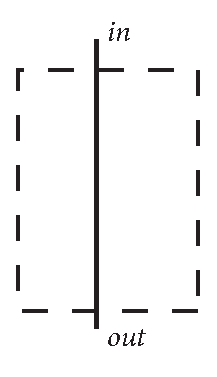
\includegraphics[scale = 0.55]{diag1}
    \caption{A simple ZX-diagram consisting of a single wire connecting input and output}
    \label{fig:diag1}
\end{figure}

A 2-qubit version would be having two wires passing through the circuit as shown in fig. \ref{fig:wires2}. This can be represented by an $I_4$ matrix $$\begin{pmatrix}
    1 & 0 & 0 & 0\\
    0 & 1 & 0 & 0\\
    0 & 0 & 1 & 0\\
    0 & 0 & 0 & 1
\end{pmatrix}.$$ 

\begin{figure}[ht]
    \centering
    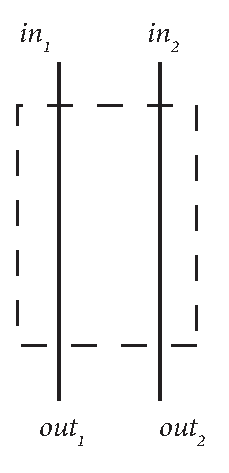
\includegraphics[scale = 0.45]{Figures/wires2-straight.eps}
    \caption{A ZX-circuit having two input/output connections.}
    \label{fig:wires2}
\end{figure}

Remember that we mentioned earlier that the shape of the wires do not matter. It is also worth noting that the overlapping paths of the wires do not matter either, hence the circuit in fig. \ref{fig:wires2-overlap} is the same as the one in fig. \ref{fig:wires2}.

\begin{figure}[ht]
    \centering
    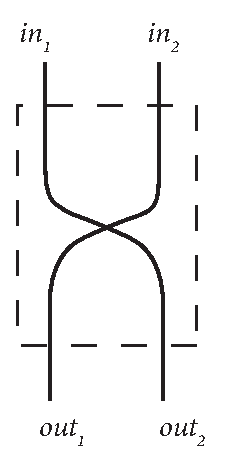
\includegraphics[scale=0.45]{wires2}
    \caption{In ZX-calculus notation, the wires can overlap without being ``shorted". Hence, this figure shows an $I_4$ circuit.}
    \label{fig:wires2-overlap}
\end{figure}

Notice the size of the matrices; the circuit with 1 wire from input to output has a matrix representation if size $2$-by$2$ while the one with two wires is 4-by-4. In fact, 

The 2-by-2 matrix represents the transformation of a 2-by-1 statevector to another 2-by-1 vector such that

\begin{align*}
    \begin{pmatrix}
        1 & 0\\
        0 & 1
    \end{pmatrix}
    \begin{pmatrix}
        \alpha \\ \beta
    \end{pmatrix}
    &= \begin{pmatrix}
        \alpha \\ \beta
    \end{pmatrix}
\end{align*}
Thus, the circuit in fig. \ref{fig:wires2} is a unitary transformation from a single-qubit statevector ($\alpha\ket{0} + \beta\ket{1}$) to another single-qubit statevector. This can be written mathematically as $\ket{\psi}\xrightarrow{}\ket{\psi}$.

You can verify this result for the 4-by-4 matrix by taking the statevector as 
$$
\begin{pmatrix}
    \alpha \\ \beta \\ \gamma \\ \delta
\end{pmatrix}.
$$

\subsection{Vertices}
But working with wires alone is no fun, right? Thus, to ``play" with qubits a bit, we can introduce vertices. These vertices allow us to perform certain operations on qubits. Of what kind? Let's explore!

Let's begin with the $H$-vertex. It is simply the Hadamard transform as discussed in the previous section with a matrix representation
$$
\dfrac{1}{\sqrt{2}}
\begin{pmatrix}
    1 & 0\\
    0 & -1
\end{pmatrix}
$$

Thus, this vertex represents a unitary transformation.

$Z_1^1$-vertex represents the $R_z(\alpha)$ transform having matrix representation
$$
\begin{pmatrix}
    1 & 0\\
    0 & e^{\iota\alpha}
\end{pmatrix}
$$
This means that the state $\ket{0}$ will remain unaffected after passing through the $Z$-vertex while the state $\ket{1}$ will gain a local phase of $\alpha$. Here, we have ignored the local phase.

\begin{table}[H]
\centering
    \begin{tabular}{llll}
        Z = $\left(\begin{matrix}
        1 & 0 \\
        0 & -1
        \end{matrix}\right)$; & & $\tikzfig{Figures/Zgate}$ & = $\tikzfig{Figures/ZgateZX}$
    \end{tabular}
    \end{table}
    
Thus, a $Z_m^n(\alpha)$-vertex can be seen a transformation of the state $\left(\cfrac{\ket{0} + \ket{1}}{\sqrt{2}}\right)^{\otimes m}$ to $\left(\cfrac{\ket{0} + e^{\iota\alpha}\ket{1}}{\sqrt{2}}\right)^{\otimes n}$.  

\begin{equation*}
\begin{tikzpicture}
    \begin{pgfonlayer}{nodelayer}
        \node [style=none] (0) at (0.00, 0.00) {};
        \node [style=none] (1) at (0.00, -1.00) {};
        \node [style=none] (2) at (0.00, -2.00) {};
        \node [style=Z dot] (3) at (1.50, -1.00) {\param{\frac{\pi}{2}}};
        \node [style=none] (4) at (3.00, -1.00) {};
        \node [style=none] (5) at (3.00, -2.00) {};
    \end{pgfonlayer}
    \begin{pgfonlayer}{edgelayer}
        \draw (0) to (3);
        \draw (1) to (3);
        \draw (2) to (3);
        \draw (3) to (4);
        \draw (3) to (5);
    \end{pgfonlayer}
\end{tikzpicture}
\end{equation*}

A last interesting case for the $Z$-vertex will be the $Z_0^1$ and $Z_1^0$ vertices. $Z_0^1(\alpha)$ is a transformation $1\xrightarrow{}\ket{0}$ and also $1\xrightarrow{}e^{\iota\alpha}\ket{1}$ (as the wire signifies a superposition state $\ket{+}$). Thus, this vertex is represented as $\dfrac{1}{\sqrt{2}}(\ket{0} + e^{\iota\alpha}\ket{1})$. In the same way, $Z_1^0(\alpha)$ vertex is a transformation $\dfrac{1}{\sqrt{2}}(\ket{0} + e^{\iota\alpha}\ket{1})\xrightarrow{}1$ and hence can be represented as  $\dfrac{1}{\sqrt{2}}(\bra{0} + e^{\iota\alpha}\bra{1})$. Notice that it is simply the transpose of $Z_0^1$ vertex. 

\begin{center}
\begin{longtable}{llll}
    $\ket{+} = \dfrac{1}{\sqrt{2}}\left(\begin{matrix}
    1 \\
    1
    \end{matrix}\right)$; & & $\ket{+}$ \textbf{---} & = $\tikzfig{Figures/ket+}$ \\[5mm]
    
    $\ket{-} = {\dfrac{1}{\sqrt{2}}}  \left(\begin{matrix}
    ~1 \\
    -1
    \end{matrix}\right)$; & & $\ket{-}$ \textbf{---} & = $\tikzfig{Figures/ket-}$
\end{longtable}
\end{center}

$X_1^1(\alpha)$-vertex represents the $R_x(\alpha)$ transform having matrix representation
$$
\begin{pmatrix}
    \cos{\frac{\alpha}{2}} & -\iota\sin{\frac{\alpha}{2}}\\
    -\iota\sin{\frac{\alpha}{2}} & \cos{\frac{\alpha}{2}}
\end{pmatrix}
$$
This means that the state $\ket{+}$ will become $\ket{-}$ after passing through the $X$-vertex while the state $\ket{-}$ will become $\ket{+}$.

\begin{center}
    \begin{longtable}{llll}
        X = $\left(\begin{matrix}
        0 & 1 \\
        1 & 0
        \end{matrix}\right)$; & & $\tikzfig{Figures/XGate}$ & = $\tikzfig{Figures/XGateZX}$
    \end{longtable}
\end{center}

Thus, an $X_m^n(\pi)$-vertex can be seen a transformation of the state $\left(\cfrac{\ket{0} + \ket{1}}{\sqrt{2}}\right)^{\otimes m}$ to $\left(\cfrac{\ket{0} - \ket{1}}{\sqrt{2}}\right)^{\otimes n}$.  

A last interesting case for the $X$-vertex will be the $X_0^1$ and $X_1^0$ vertices. $X_0^1(\alpha)$ is a transformation $1\xrightarrow{}(\cos(\frac{\alpha}{2}) - \iota\sin(\frac{\alpha}{2}))\ket{0}$ and also $1\xrightarrow{}(\cos(\frac{\alpha}{2}) - \iota\sin(\frac{\alpha}{2}))\ket{1}$ (as the wire signifies a superposition state $\ket{+}$). Thus, this vertex is represented as $$\dfrac{(\cos(\frac{\alpha}{2}) - \iota\sin(\frac{\alpha}{2}))}{\sqrt{2}}(\ket{0} + \ket{1})$$. In the same way, $X_1^0(\alpha)$ vertex is a transformation $\dfrac{(\cos(\frac{\alpha}{2}) - \iota\sin(\frac{\alpha}{2}))}{\sqrt{2}}(\ket{0} + \ket{1})\xrightarrow{}1$ and hence can be represented as  $\dfrac{(\cos(\frac{\alpha}{2}) - \iota\sin(\frac{\alpha}{2}))}{\sqrt{2}}(\bra{0} + \bra{1})$. Notice that it is simply the transpose of $X_0^1$ vertex. 

\begin{center}
\begin{longtable}{llll}
    $\ket{0}$ = $\left(\begin{matrix}
    1  \\
    0
    \end{matrix}\right)$; & & $\ket{0}$ \textbf{---} & = $\tikzfig{Figures/ket0}$ \\[5mm]
    
    $\ket{1}$ = $\left(\begin{matrix}
    0\\
    1
    \end{matrix}\right)$; & & $\ket{1}$ \textbf{---} & $= \tikzfig{Figures/ket1}$ 
\end{longtable}
\end{center}

% \pagebreak
% \hline

% And the quantum gates in ZX-Calculus are described as follows

% \begin{center}
% \begin{longtable}{llll}
%     H = $\dfrac{1}{\sqrt{2}}
%     \left(\begin{matrix}
%     1 & 1 \\
%     1 & -1
%     \end{matrix}\right)$; & & $\tikzfig{Figures/Hgate}$ & = $\tikzfig{Figures/HgateZX}$ \\[5mm]
    
%     Z = $\left(\begin{matrix}
%     1 & 0 \\
%     0 & -1
%     \end{matrix}\right)$; & & $\tikzfig{Figures/Zgate}$ & = $\tikzfig{Figures/ZgateZX}$ \\ [5mm]
    
%     CNOT = $\left(\begin{matrix}
%     1 & 0 & 0 & 0 \\
%     0 & 1 & 0 & 0 \\
%     0 & 0 & 0 & 1 \\
%     0 & 0 & 1 & 0 \\
%     \end{matrix}\right)$; & & $\tikzfig{Figures/CNOTgate}$ & = $\tikzfig{Figures/CNOTgateZX}$\\ [5mm]
    
%     SWAP = $\left(\begin{matrix}
%     1 & 0 & 0 & 0 \\
%     0 & 0 & 1 & 0 \\
%     0 & 1 & 0 & 0 \\
%     0 & 0 & 0 & 1 \\
%     \end{matrix}\right)$; & & $\tikzfig{Figures/SWAPgate}$ & = $\tikzfig{Figures/SWAPgateZX}$
% \end{longtable}
% \end{center}
\chapter{PyZX: ZX-Calculus Using Python}
\label{ch:pyzx}

% \section{So, What is PyZX?}
Now that we have a basic understanding about ZX-Calculus, we can now take our knowledge a step further into a more computational approach. Since we have already installed PyZX as a package in the previous chapter, we will dive more into quantum circuits and how this library works.

\large{PyZX} is a Python-based library designed with the purpose of reasoning with large {quantum circuits} and {ZX-diagrams}. Luckily for us, it is  an open-source resource -- and completely free! With PyZX, we can efficiently rewrite ZX-diagrams using some simplification strategies. And don't think these "strategies" are not that important -- they are so powerful that they are able to perform highly effective T-count optimization and even to verify correctness of optimised circuits. 

If you think that's {not enough}, PyZX also offers diverse ways to visualise circuits and ZX-diagrams. With this tool, we will be able to present circuits in QC, QASM and Quipper formats, and it can also convert ZX-diagrams into TikZ diagrams. In short, PyZX is a really powerful tool for circuit optimization; for example, to optimize multiple circuits or combining these with other external procedures. 

\section{Overview}
We will now specify the main features of PyZX and how you can implement them. The objective of this section is not to give a detailed tutorial, but rather a brief tour of what PyZX can do. If you are interested in deepening the concepts presented, that's completely fine! We will provide resources for further study in the last section of the chapter. 

\subsection{ZX-diagrams and circuits}
There are two main data-structures present in PyZX: \texttt{Circuits} and \texttt{Graphs}. A \texttt{Circuit} is a wrapper around a list of gates, while a \texttt{Graph} represents a ZX-diagram.

\subsubsection{\texttt{Circuit} class}
To be more precise, the \texttt{Circuit} class is the entry-point for importing and exporting circuits to and from PyZX. There are also multiple ways to implement optimization schemes that directly act onto the \texttt{Circuit} (however, we will explain that in the "Circuit Optimisation" chapter). So, to wrap the definition up, a \texttt{Circuit} is a list of \texttt{Gates} that can be converted into various representations, like ZX-diagrams or the QASM format. The way to import a circuit into PyZX is the following:
\begin{minted}{python}
circuit = zx.Circuit.load("path/to/circuit.extension")
\end{minted}

With this, PyZX will automatically try to figure out in which format the circuit is represented! There is also a way to generate random circuits:
\begin{minted}{python}
>>> circuit = zx.generate.CNOT_HAD_PHASE_circuit(qubits=10,depth=20,clifford=True)
\end{minted}

Also, if you use \texttt{zx.draw}, a matplotlib figure would be returned instead. 

\begin{figure}[H]
        \centering
        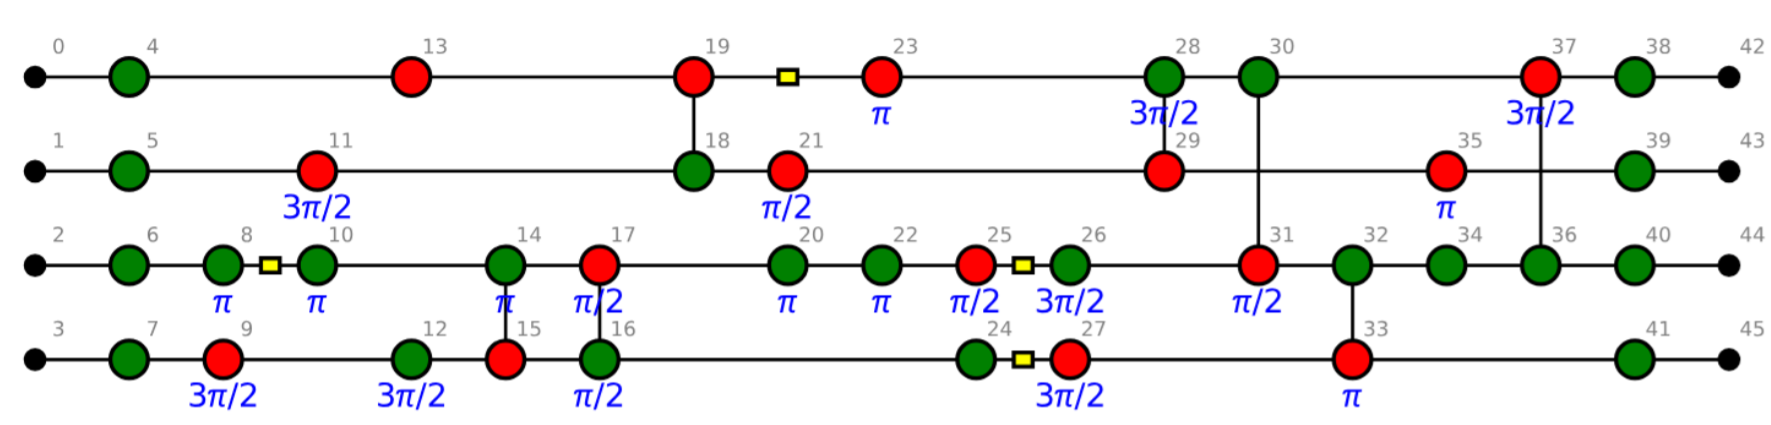
\includegraphics[width = 0.9\textwidth]{Figures/examplepyzx.png}
        \caption{Example of the default drawing method of quantum circuits.}
        \label{fig:diagram-ex}
    \end{figure}

You can also convert a circuit into a ZX-diagram:
\begin{minted}{python}
g = circuit.to_graph()
\end{minted}

To explain in further depth the simplification routines of ZX-diagrams, we will use a built-in example:
\begin{minted}{python}
zx.clifford_simp(g)  #simplifies the diagram with the clifford_simp method
g.normalize()        #makes it more presentable
zx.draw(g)
\end{minted}

\begin{figure}[ht]
        \centering
        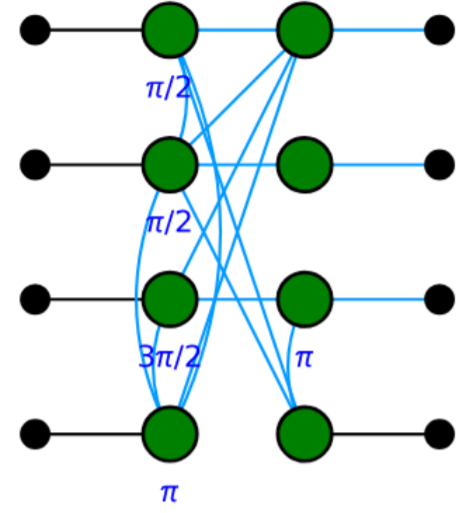
\includegraphics[scale = 0.5]{Figures/companentex.png}
        \caption{A new more compact form of the example above. The blue lines represent edges which have a Hadamard gate on them.}
        \label{fig:diagram-ex}
    \end{figure}

Internally, a ZX-diagram is represented as a \textbf{graph}.

\subsubsection{\texttt{Graph} class}
The \texttt{Graph} class is much more interesting. As you could see in the previous chapter, the graphs in PyZX are pretty simple graphs with typed vertices and edges. There are three types of vertices: boundaries, Z-spiders, and X-spiders. Every single vertex can be labelled by a phase that is stored as a fraction representing a rational multiple of $\pi$. These edges can also be divided in two types: one with a regular connection between spiders and a Hadamard-edge. 

One of the most common things to deal with PyZX graphs in ZX-Calculus is to add an edge. This can be done with the \texttt{$add\_edge$} method. However, if we add an edge where there is already one present will simply replace it. Because of this, it is sometimes more convenient to use the rules of ZX-Calculus to resolve parallel edges and self-loops whenever a new edge is added. And to use this functionality, we can use the \texttt{Graph} method \texttt{$add\_edge\_table$}, which will take in a list of edges and edge-types to then resolve how the ZX-diagram would look like when every single self-loop or double edges have been resolved. 

The \texttt{Graph} class

\section{Manually constructing an ZX-diagram}

\section{Further Resources}
As promised, we included some sources so you can deepen your knowledge in the presented information. 

\chapter{Quantum Circuit Optimisation}
As we saw in the previous chapters, PyZX works with quantum circuits, which are a kind of assembly language in quantum computation. They consist of primitive quantum operations (more commonly known as \textbf{gates}) applied in sequence to some quantum data (you know the drill). 

Gates take time and produce noise. So if we could do the same tasks but with \textit{fewer} gates, we win. This concept is called \textbf{quantum circuit optimisation}.

In Chapter 5, we learned how to \textbf{simplify} quantum circuits. This is, indeed, a method of optimization. And to transform these type of circuits into another with this method, we can use \textbf{spiders}.

\section{Optimisation with spiders}
Sometimes things get messy as circuits are \textit{very} rigid. Because of this, we use ZX-diagrams to simplify them! 

There's another method we could do: divide gates into smaller pieces called \textbf{spiders}. These spiders satisfy \textbf{eight} equations, which in short are called the \textbf{ZX Calculus}. In other words, \textbf{what gates are to circuits, spiders are to ZX-diagrams}. 

\begin{figure}[H]
        \centering
        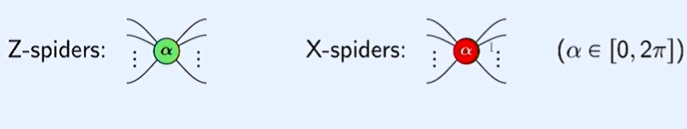
\includegraphics[width=0.5\textwidth]{Figures/spiderspic.png}
        \caption{Example of Z-spider and X-spider.}
        \label{fig:spiders.picture}
    \end{figure}
There are two types types of spiders: Z-spiders and X-spiders. They are always denoted with both colors: green and red. Now you may already understand the reason of our app's logo! 

Contrary to a quantum circuit, we can wire spiders in any way or shape you want. Therefore, \textbf{only connectivity matters}.
\begin{figure}[H]
        \centering
        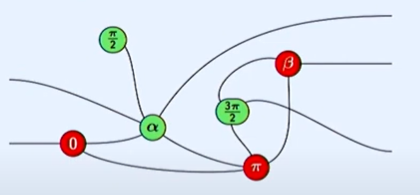
\includegraphics[width=0.5\textwidth]{Figures/example.spiders.png}
        \caption{Example of a quantum circuit using spiders.}
        \label{fig:spiders.picture}
    \end{figure}

For example, in this circuit, there are two qubits as an input and three qubits as an output. Note that we can write \textit{any} quantum gate as a ZX-diagram, so there are no excuses! Below we specify the equivalences of each gate to a spider:
\begin{figure}[H]
        \centering
        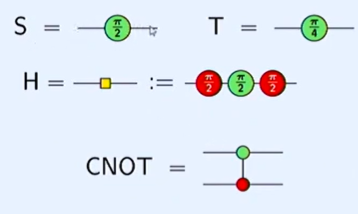
\includegraphics[width=0.5\textwidth]{Figures/equivalence.spiders.png}
        \caption{Important equivalences between gates and spiders.}
        \label{fig:eq.spiders}
    \end{figure}
So, if you remember the basics of quantum mechanics, the S gate does a quarter rotation to the qubit. $\frac{\pi}{2}$ is like a quarter rotational space ($\frac{180°}{2} = 90^\circ$, which is a quarter of 360$^\circ$). The T gate is a $\frac{1}{8}$ rotation so the spider we use is $\frac{\pi}{4}$. The Hadamard gate, on the other hand, can be decomposed in three basic rotations ($\frac{\pi}{2}$, $\frac{\pi}{2}$, $\frac{\pi}{2}$). To make this easier to read, we only use a yellow square to represent the three operations made in the qubit. Finally, the CNOT gate is solely a composition of two spiders. These are just some examples of how you can "translate" gates into spiders (actually, it was a refresher of the ZX-intro chapter). 

In the previous chapter, we could also see the rules of ZX-diagrams. Before moving on to optimisation, it is extremely important to note that if two ZX-diagrams represent the same computation, then they can be transformed into one another using the eight previous rules explained. So, instead of having dozens of \textbf{dozens} of circuit equalities, we have it much more simple now with a few simple rules! That's why ZX-Calculus is so important. The spiders "chop out" the gates in the circuit. Then, PyZX reduces it automatically using the ZX Calculus and that's it! You have successfully optimized your quantum circuit with spiders.

\begin{figure}[H]
        \centering
        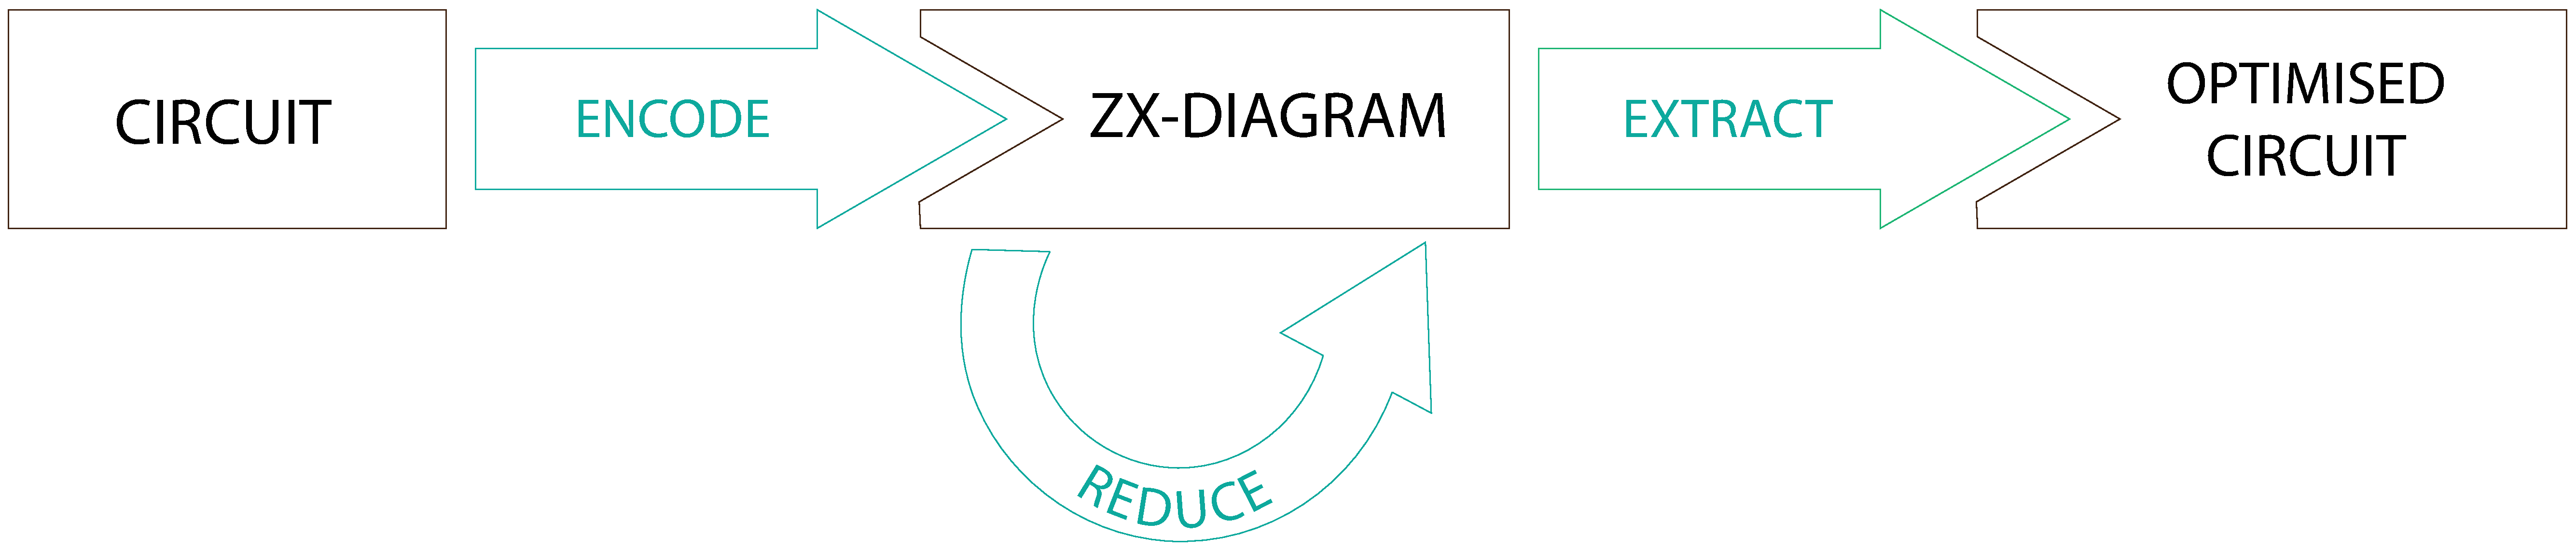
\includegraphics[width = 0.95\textwidth]{Figures/optimisation-roadmap.eps}
        \caption{ZX-diagram overall functioning}
        \label{fig:def-pyzx}
    \end{figure}

That is the main argument of ZX Calculus optimization. It is important to note that this is just an \textit{introduction} to the topic, hence we will not explain in depth the mathematics behind. However, we will be adding this material so everyone can learn it from scratch in another opportunity!

\section{Equational Rules}
\subsection{T-Rule}
The most simple way to describe it is with the concept of "only the topology matters". When spiders are in a quantum circuit, the wires may be arbitrarily organized. Still, this doesn't affect the overall computation of the program. By enumerating the inputs and outputs, any topological deformation in the middle can be simplified in a simple line. In other words, wires can be stretched or bent without consequence. If the concept doesn't "click" in your head immediately, don't worry! Here is a more visual explanation.
\begin{figure}[H]
        \centering
        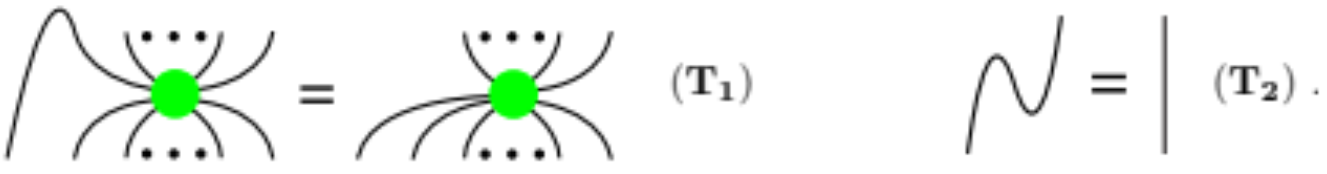
\includegraphics[width = 0.95\textwidth]{Figures/t.rule.ex.png}
        \caption{The two T-rules, T1 and T2.}
        \label{fig:t1-t2}
    \end{figure}

\begin{center}
\fcolorbox{black}{shadecolor}{%

    \parbox{\textwidth}
    {%
        \small
        {
            \textbf{Important!}
            Even though the slogan says "only the topology matters", this does NOT mean that the topology is always preserved. In fact, if you simplify a circuit, the topology will vary. The rules that we will explain may change the topology of the circuit by removing loops or even disconnecting previously connected vertices.
        }
    }%
}
\end{center}

\subsection{S-Rule}
Stands for the "spider" rule. These rules explain how dots of the \textbf{same color} interact. We have two rules:
\subsubsection{S1}
Rule S1 states that if dots of the same color are connected, they can be merged, summing the phases. Conversely, a dot can be decomposed along one or more connecting wires. Here we have a picture that illustrates the process.

\begin{figure}[H]
        \centering
        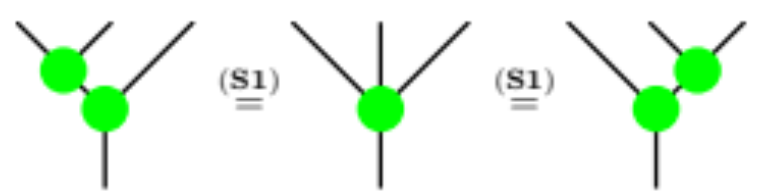
\includegraphics[width = 0.95\textwidth]{Figures/Screenshot (33).png}
        \caption{The S1 rule.}
        \label{fig:s1-rule}
    \end{figure}

\subsubsection{S2}
Rule S2 specifies when spiders are trivial. In other words, dots of degree 2 with phase $\alpha$ = 0 can be removed or, conversely, introduced.  

\subsection{B-Rule}

\subsection{K-Rule}

\subsection{C-Rule}

\subsection{D-Rule}

%-----------------------------------------------------------------------
\pagestyle{empty}
\afterpage{\null\newpage}
%-----------------------------------------------------------------------


\bibliographystyle{unsrt}
\bibliography{references}

\end{document}